\documentclass[degree=bachelor,tocarialchapter]{thuthesis}
% 选项
%   degree=[bachelor|master|doctor|postdoctor], % 必选,学位类型
%   language=[chinese|english], % 可选(默认:chinese),论文的主要语言
%   secret,                % 可选(默认:关闭),是否有密级
%   tocarialchapter,       % 可选(默认:关闭),章目录中使用黑体(这项表示同时打开下面两项)
%   tocarialchapterentry,  % 可选(默认:关闭),单独控制章标题在目录中使用黑体
%   tocarialchapterpage,   % 可选(默认:关闭),单独控制章页码在目录中使用黑体

% 所有其它可能用到的包都统一放到这里了,可以根据自己的实际添加或者删除。
\usepackage{thuthesis}

\newcommand{\mbi}{\mathbb{I}}
% \usepackage{unicode-math}
% \setmathfont{libertinusmath-regular.otf}
% \newtheorem{theorem}{Theorem}[section]
% \newtheorem{lemma}[theorem]{Lemma}
% \newtheorem{proposition}[theorem]{Proposition}
% \newtheorem{corollary}[theorem]{Corollary}
% \newtheorem{definition}[theorem]{Definition}
% \newtheorem{assertion}[theorem]{Assertion}
% \newtheorem{assumption}[theorem]{Assumption}
% 定义所有的图片文件在 figures 子目录下
\graphicspath{{figures/}}

% 可以在这里修改配置文件中的定义。导言区可以 使用中文。
% \def\myname{薛瑞尼}

\begin{document}

%%% 封面部分
\frontmatter
\thusetup{
  %******************************
  % 注意:
  %   1. 配置里面不要出现空行
  %   2. 不需要的配置信息可以删除
  %******************************
  %
  %=====
  % 秘级
  %=====
  secretlevel={秘密},
  secretyear={10},
  %
  %=========
  % 中文信息
  %=========
  ctitle={卷积神经网络理论综述},
  cdegree={本科},
  cdepartment={土木工程},
  cmajor={土木工程},
  cauthor={谭泽人},
  csupervisor={史作强副教授},
  cassosupervisor={包承龙助理教授}, % 副指导老师
  ccosupervisor={某某某教授}, % 联合指导老师
  % 日期自动使用当前时间,若需指定按如下方式修改:
  % cdate={超新星纪元},
  %
  % 博士后专有部分
  catalognumber     = {分类号},  % 可以留空
  udc               = {UDC},  % 可以留空
  id                = {编号},  % 可以留空: id={},
  cfirstdiscipline  = {计算机科学与技术},  % 流动站(一级学科)名称
  cseconddiscipline = {系统结构},  % 专 业(二级学科)名称
  postdoctordate    = {2009 年 7 月——2011 年 7 月},  % 工作完成日期
  postdocstartdate  = {2009 年 7 月 1 日},  % 研究工作起始时间
  postdocenddate    = {2011 年 7 月 1 日},  % 研究工作期满时间
  %
  %=========
  % 英文信息
  %=========
  etitle={An Introduction to \LaTeX{} Thesis Template of Tsinghua University v\version},
  % 这块比较复杂,需要分情况讨论:
  % 1. 学术型硕士
  %    edegree:必须为Master of Arts或Master of Science(注意大小写)
  %             “哲学、文学、历史学、法学、教育学、艺术学门类,公共管理学科
  %              填写Master of Arts,其它填写Master of Science”
  %    emajor:“获得一级学科授权的学科填写一级学科名称,其它填写二级学科名称”
  % 2. 专业型硕士
  %    edegree:“填写专业学位英文名称全称”
  %    emajor:“工程硕士填写工程领域,其它专业学位不填写此项”
  % 3. 学术型博士
  %    edegree:Doctor of Philosophy(注意大小写)
  %    emajor:“获得一级学科授权的学科填写一级学科名称,其它填写二级学科名称”
  % 4. 专业型博士
  %    edegree:“填写专业学位英文名称全称”
  %    emajor:不填写此项
  edegree={Doctor of Engineering},
  emajor={Computer Science and Technology},
  eauthor={Xue Ruini},
  esupervisor={Professor Zheng Weimin},
  eassosupervisor={Chen Wenguang},
  % 日期自动生成,若需指定按如下方式修改:
  % edate={December, 2005}
  %
  % 关键词用“英文逗号”分割
  ckeywords={TeX, LaTeX, CJK, 模板, 论文},
  ekeywords={TeX, LaTeX, CJK, template, thesis}
}

% 定义中英文摘要和关键字
\begin{cabstract}
  论文的摘要是对论文研究内容和成果的高度概括。摘要应对论文所研究的问题及其研究目
  的进行描述,对研究方法和过程进行简单介绍,对研究成果和所得结论进行概括。摘要应
  具有独立性和自明性,其内容应包含与论文全文同等量的主要信息。使读者即使不阅读全
  文,通过摘要就能了解论文的总体内容和主要成果。

  论文摘要的书写应力求精确、简明。切忌写成对论文书写内容进行提要的形式,尤其要避
  免“第 1 章……;第 2 章……;……”这种或类似的陈述方式。

  本文介绍清华大学论文模板 \thuthesis{} 的使用方法。本模板符合学校的本科、硕士、
  博士论文格式要求。

  本文的创新点主要有:
  \begin{itemize}
    \item 用例子来解释模板的使用方法;
    \item 用废话来填充无关紧要的部分;
    \item 一边学习摸索一边编写新代码。
  \end{itemize}

  关键词是为了文献标引工作、用以表示全文主要内容信息的单词或术语。关键词不超过 5
  个,每个关键词中间用分号分隔。(模板作者注:关键词分隔符不用考虑,模板会自动处
  理。英文关键词同理。)
\end{cabstract}

% 如果习惯关键字跟在摘要文字后面,可以用直接命令来设置,如下:
% \ckeywords{\TeX, \LaTeX, CJK, 模板, 论文}

\begin{eabstract}
   An abstract of a dissertation is a summary and extraction of research work
   and contributions. Included in an abstract should be description of research
   topic and research objective, brief introduction to methodology and research
   process, and summarization of conclusion and contributions of the
   research. An abstract should be characterized by independence and clarity and
   carry identical information with the dissertation. It should be such that the
   general idea and major contributions of the dissertation are conveyed without
   reading the dissertation.

   An abstract should be concise and to the point. It is a misunderstanding to
   make an abstract an outline of the dissertation and words ``the first
   chapter'', ``the second chapter'' and the like should be avoided in the
   abstract.

   Key words are terms used in a dissertation for indexing, reflecting core
   information of the dissertation. An abstract may contain a maximum of 5 key
   words, with semi-colons used in between to separate one another.
\end{eabstract}

% \ekeywords{\TeX, \LaTeX, CJK, template, thesis}

% 如果使用授权说明扫描页,将可选参数中指定为扫描得到的 PDF 文件名,例如:
% \makecover[scan-auth.pdf]
\makecover

%% 目录
\tableofcontents

%% 符号对照表
\begin{denotation}[3cm]
\item[HPC] 高性能计算 (High Performance Computing)
\item[cluster] 集群
\item[Itanium] 安腾
\item[SMP] 对称多处理
\item[API] 应用程序编程接口
\item[PI] 聚酰亚胺
\item[MPI] 聚酰亚胺模型化合物,N-苯基邻苯酰亚胺
\item[PBI] 聚苯并咪唑
\item[MPBI] 聚苯并咪唑模型化合物,N-苯基苯并咪唑
\item[PY] 聚吡咙
\item[PMDA-BDA]	均苯四酸二酐与联苯四胺合成的聚吡咙薄膜
\item[$\Delta G$] 活化自由能 (Activation Free Energy)
\item[$\chi$] 传输系数 (Transmission Coefficient)
\item[$E$] 能量
\item[$m$] 质量
\item[$c$] 光速
\item[$P$] 概率
\item[$T$] 时间
\item[$v$] 速度
\item[劝学] 君子曰:学不可以已。青,取之于蓝,而青于蓝;冰,水为之,而寒于水。木
  直中绳。輮以为轮,其曲中规。虽有槁暴,不复挺者,輮使之然也。故木受绳则直,金就
  砺则利,君子博学而日参省乎己,则知明而行无过矣。吾尝终日而思矣,不如须臾之所学
  也;吾尝跂而望矣,不如登高之博见也。登高而招,臂非加长也,而见者远;顺风而呼,
  声非加疾也,而闻者彰。假舆马者,非利足也,而致千里;假舟楫者,非能水也,而绝江
  河,君子生非异也,善假于物也。积土成山,风雨兴焉;积水成渊,蛟龙生焉;积善成德,
  而神明自得,圣心备焉。故不积跬步,无以至千里;不积小流,无以成江海。骐骥一跃,
  不能十步;驽马十驾,功在不舍。锲而舍之,朽木不折;锲而不舍,金石可镂。蚓无爪牙
  之利,筋骨之强,上食埃土,下饮黄泉,用心一也。蟹六跪而二螯,非蛇鳝之穴无可寄托
  者,用心躁也。—— 荀况
\end{denotation}



% % 也可以使用 nomencl 宏包:

% \printnomenclature[3cm]

% \nomenclature{HPC}{高性能计算 (High Performance Computing)}
% \nomenclature{cluster}{集群}
% \nomenclature{Itanium}{安腾}
% \nomenclature{SMP}{对称多处理}
% \nomenclature{API}{应用程序编程接口}
% \nomenclature{PI}{聚酰亚胺}
% \nomenclature{MPI}{聚酰亚胺模型化合物,N-苯基邻苯酰亚胺}
% \nomenclature{PBI}{聚苯并咪唑}
% \nomenclature{MPBI}{聚苯并咪唑模型化合物,N-苯基苯并咪唑}
% \nomenclature{PY}{聚吡咙}
% \nomenclature{PMDA-BDA}{均苯四酸二酐与联苯四胺合成的聚吡咙薄膜}
% \nomenclature{$\Delta G$}{活化自由能 (Activation Free Energy)}
% \nomenclature{$\chi$}{传输系数 (Transmission Coefficient)}
% \nomenclature{$E$}{能量}
% \nomenclature{$m$}{质量}
% \nomenclature{$c$}{光速}
% \nomenclature{$P$}{概率}
% \nomenclature{$T$}{时间}
% \nomenclature{$v$}{速度}



%%% 正文部分
\mainmatter
\chapter{背景介绍}
\label{cha:intro}

在介绍卷积神经网络(Convolutional Neural Network,简称为  CNN)的相关理论结果之前,我们先对卷积神经网络的发展,卷积神经网络的应用成果以及卷积神经网络的工作方式进行一定的介绍。

\section{卷积神经网络的发展历史}
对于CNN的提出有重大影响的工作最早可以追溯到1968年Hubel和Wiesel的一次对猫的视觉反应的观察实验。他们将示波器连接到猫的视觉神经上,观察猫在看到不同图像时,示波器的波形的变化。他们的实验发现视觉的处理过程中,部分输入信息被丢失,多个输入对应到了同一个输出,也就是说,部分信息被神经元“过滤”了。因为这项工作Hubel和Wiesel共享了1981年诺贝尔奖。而在1980年,日本科学家Kunihiko Fukishima(福岛邦彦)受到Hubel和Wiesel实验的启发,发表了题为《Neocognitron: A self-organizing neural network model for a mechanism of pattern recognition unaffected by shift in position》的论文\cite{fukushima1980neocognitron},提出了Neocongnitron。这篇工作中,Kunihiko Fukishima在人工神经网络中引入了人类视觉系统的概念,提出了现在成为卷积和池化的概念,普遍认为这是现在CNN的雏形。
\par
在之后的大约十年内,虽然有很多研究者基于Kunihiko Fukishima的Neocognitron提出了一些模型,但是都没有大的突破,直到1989年,Yann LeCun在《Backpropagation applied to handwritten zip code recognition》 \cite{lecun1989backpropagation}中吸取了Neocognitron的核心思想,并且引入了LeCun在Back Propogation方面的工作。在这篇论文中LeCun定义了新的卷积操作,使得网络的泛化能力提高,训练速度也加快。
\par
1998年,\citet{lecun1998gradient}提出了LeNet-5,这时的LeNet-5与现在的CNN的结构基本一致,只是在最后一层输出层,LeNet-5没有使用Fully Connected Layer,而是RBF Layer。LeNet-5的出现使得CNN的使用出现了一次高潮,但是由于计算能力的限制,与现在的应用水平相比还相去甚远。
\par
2006年,\citet{bouvrie2006notes}给出了CNN的推导和实现公式,而在之后的几年内,关于CNN的工作没有较大的突破。直到2012年,深度学习三巨头之一的Geoffrey Hinton的团队提出了基于CNN的深度神经网络AlexNet。AlexNet在ImageNet LSVRC-2012分类任务上以压倒性优势获得了最高的准确率。AlexNet的出现使得人们认识到了CNN在图像任务上的优势,在之后的几年里,不断有基于CNN的神经网络被提出,例如2013年提出的VGG\cite{simonyan2014very}和2014年提出的GoogleNet\cite{szegedy2015going},他们在ImageNet LSVRC上的表现都已经远超AlexNet,但是首次实现神经网络的识别准确率高于人类的模型是2016年\citet{he2016deep}提出的ResNet。ResNet将神经网络的深度提高了一个数量级,大大加快了神经网络的训练速度,并且提高了神经网络的识别准确率。在这之前还有很多基于CNN的网络被研究者提出,但是他们的贡献不是很突出,例如Fast RCNN\cite{girshick2015fast},SPP Net\cite{he2015spatial}等。
\begin{figure}
\centering
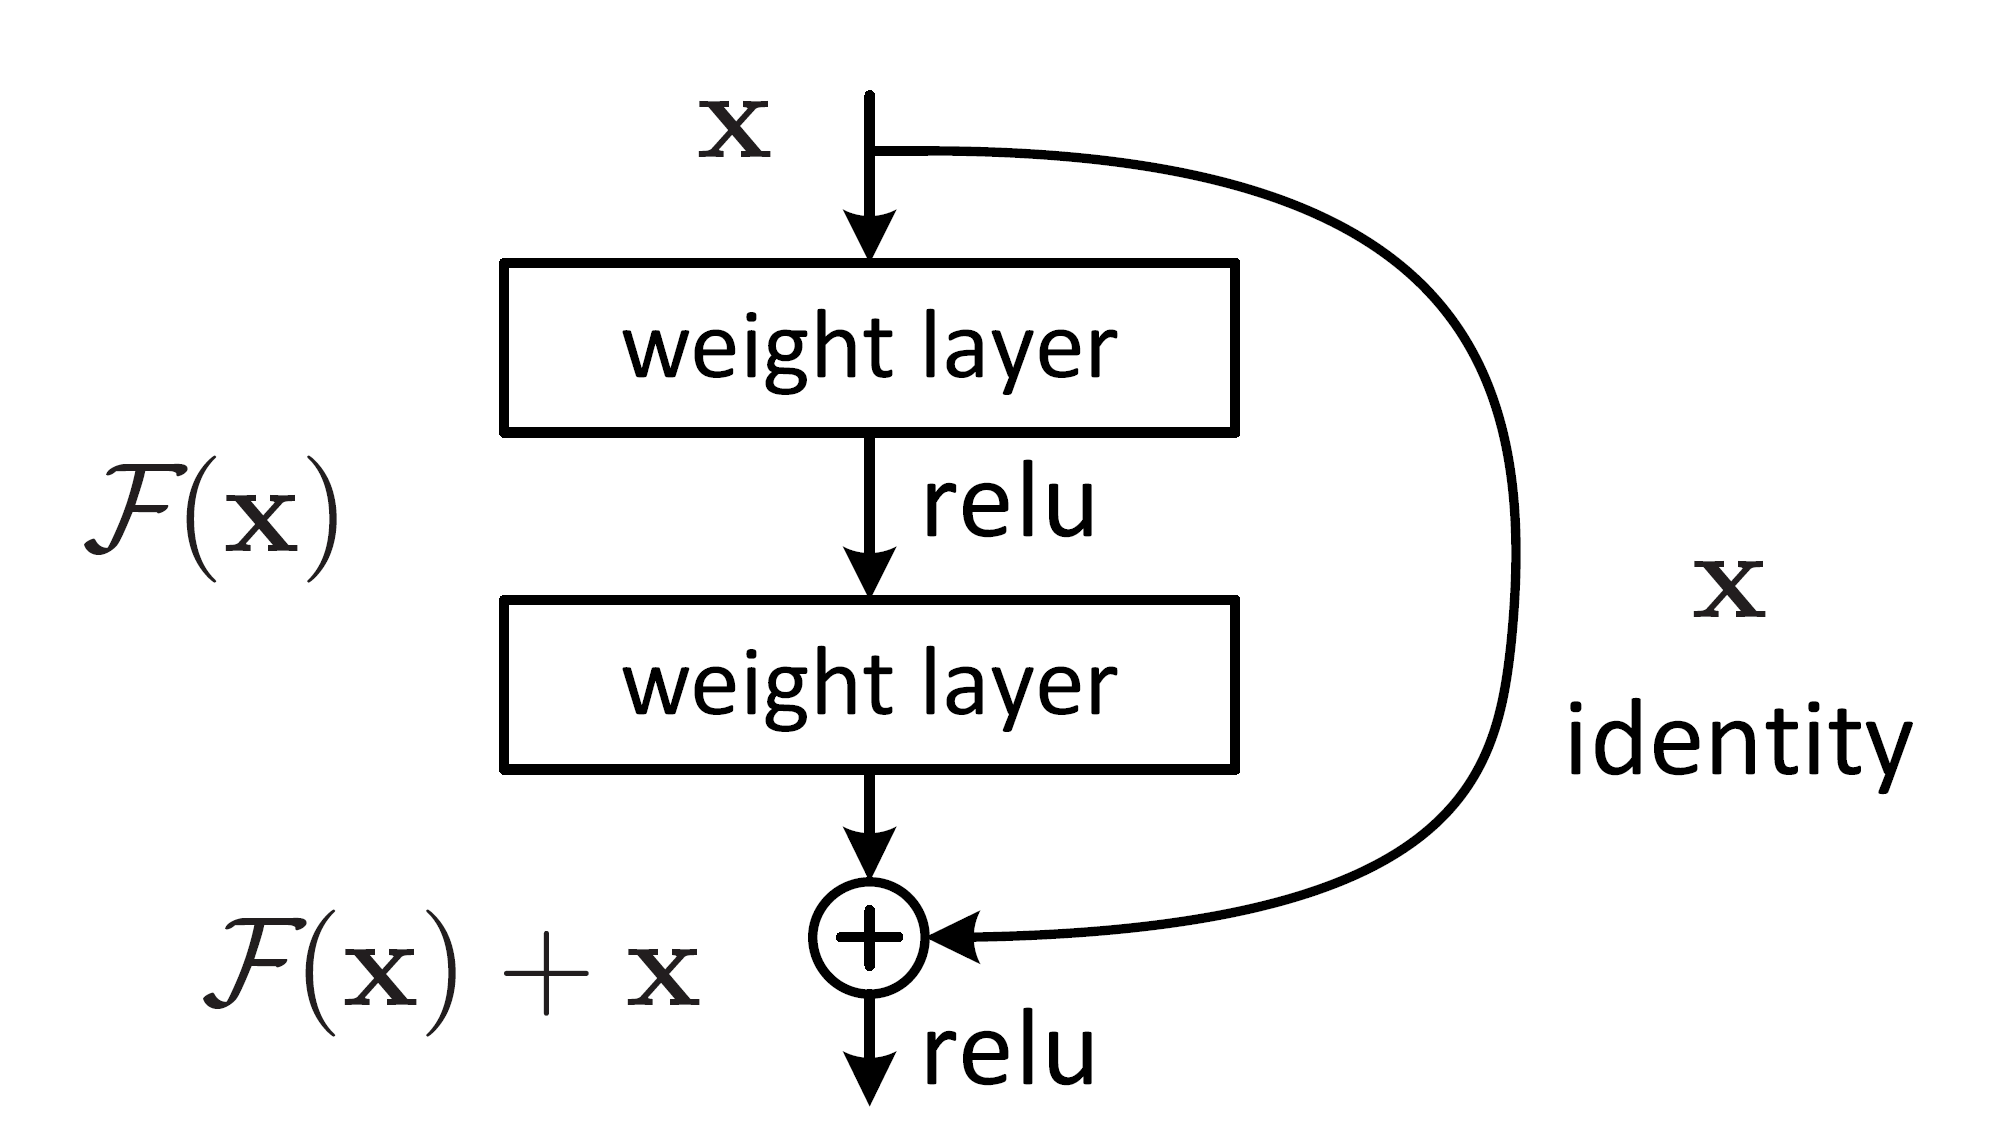
\includegraphics[width=10cm]{./figures/ResNet.PNG}
\caption{ResNet的结构\cite{he2016deep}}
\label{fig:Res}
\end{figure}


\section{卷积神经网络的工作过程}
卷积神经网络一般由卷积层,池化层,全连接层,激活层组成。简要的说,卷积层是将输入的数据信息进行过滤,池化层是对输入数据进行压缩,激活函数则是为了引入非线性而加入网络中的函数,全连接层往往用在最后一层,将卷积和池化后的数据对应到输出。下面,本文将详细的说明卷积神经网络层和池化层在处理图像数据时的作用。
\begin{itemize}
  \item 卷积层:卷积层是通过一个滤波器(卷积核),将滤波器覆盖输入的数据,并进行窗口移动,每次都与覆盖的数据进行元素间的相乘,并将相乘结果相加除以元素个数得到该窗口对应的输出值。具体说来,假设输入数据为$x\in \mathbb{R}^{n\times n}$, 滤波器为$f\in \mathbb{R}^{l\times l}$, 则输出$y\in \mathbb{R}^{(n-l+1)\times (n-l+1)}$,其中
  \[
    y_{i,j} = \frac{1}{l^2}\sum_{s = j}^{j+l-1}\sum_{t = i}^{i+l-1} x_{t,s}f_{t-i+1,s-i+1}
  \]
  \par
  图~\ref{fig:conv}~是上述过程的一个直观的说明图。
  \begin{figure}
  \centering
  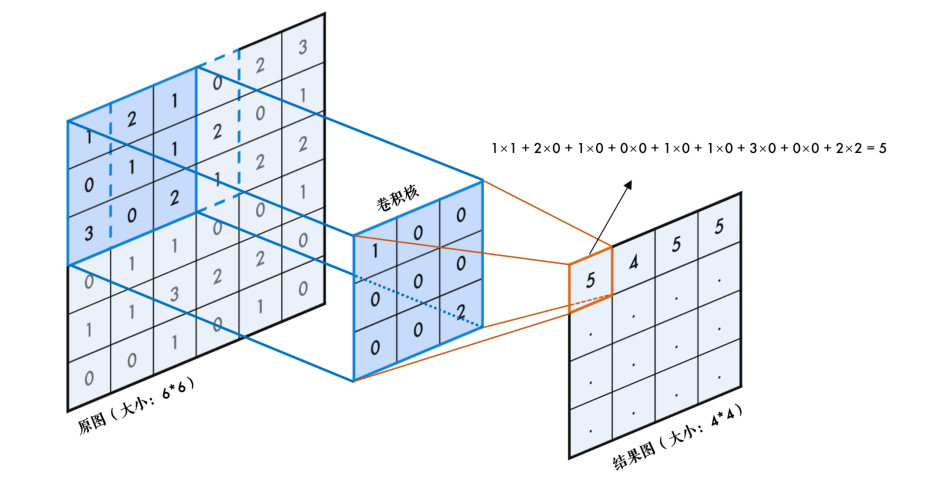
\includegraphics[width=10cm]{./figures/conv.jpg}
  \caption{卷积层工作原理示意}
  \label{fig:conv}
  \end{figure}
  \par
  卷积实际上就是计算卷积核与窗口数据之间的相似程度,但是当卷积核窗口移动时,相邻窗口之间有很多部分是重叠的,这就意味着最后的输出中有大量的重复的信息,这样的重复信息大大增加了计算的难度并且降低了计算效率。而这些重复的信息,实际上并不是需要的,神经网络需要一种机制对重复信息进行舍弃,这就是池化层的功能。
  \item 池化层:	池化层有很多种,这里我们以平均池化为例进行介绍。假设池化层的输入为$x\in \mathbb{R}^{m\times m}$,池化窗口为$d\times d$,为了简单起见,进一步假设$m\equiv 0 (\mod d)$,这个假设只是为了叙述方便,不会对结果有本质影响。
  \par
  池化层的输出为$y\in \mathbb{R}^{k\times k}$,其中$k = m/d$,且
  \[
  	y_{i,j} = \frac{1}{d^2}\sum_{s=(i-1)d+1}^{id}\sum_{t=(j-1)d+1}^{jd}x_{s,t}
  \]
  \par
  图~\ref{fig:avgpool}~展示了以$2\times2$为单位进行平均池化的一个实例。
  \begin{figure}
  \centering
  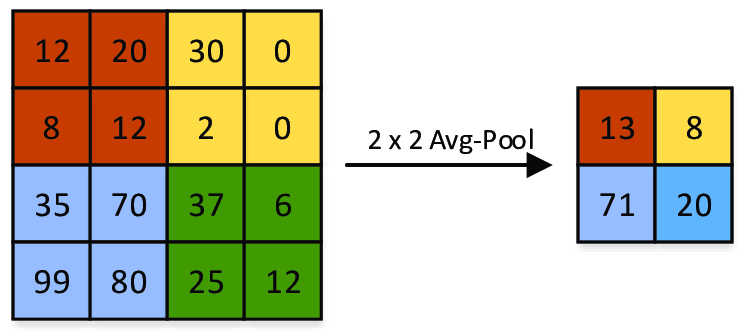
\includegraphics[width=10cm]{./figures/avgpool.png}
  \caption{平均池化的实例}
  \label{fig:avgpool}
  \end{figure}
  \par
  池化层的重要意义在于,它可以将数据进行降维,图像数据往往维度都很大,计算量很大,而进行降维可以大大降低计算量。另一方面,由于池化具有平移不变性,当输入数据受到微小扰动时,池化层的输出也会保持不变,神经网络的鲁棒性(Robustness)增强了。
\end{itemize}
\chapter{全连接神经网络理论}
在介绍卷积神经网络的理论之前,本文先介绍全连接神经网络的理论分析结果。本文按照神经网络的层数进行结果总结,并给出考虑不同的损失函数时的结果的对比。

\section{神经网络中的重要理论问题}
深度学习在诸多领域展现出卓越的效果,在许多方面已经超过了人类的水平。现实中,人们趋于在计算能力允许的情况下,使用更深更宽的神经网络,并且实验结果也表明,这样的结果会更好,但是相关的理论解释却一直都欠缺。近些年来,对深度学习的理论研究逐渐增多,	人们对于神经网络的认识逐渐深入。实际使用中的大多数神经网络中的参数数量都远大于用于训练的数据量(称为过参数化神经网络),即使有如此多的参数需要优化,神经网络在训练和测试上的误差都很小。甚至\citet{zhang2016understanding}通过实验表明,即使数据的标签被随机生成的标签替换,过参数化神经网络也可以很好的拟合数据,得到很小的训练误差,虽然在这种情况下,神经网络在测试集上的表现很差。这引起了神经网络理论研究者对两个问题广泛的谈论:1)为什么神经网络的训练误差可以很小,即使数据的标签是随机标签也可以很好的拟合?2)为什么在随机生成的标签数据上训练的神经网络的泛化能力很差,而在真实标签数据训练后的模型的泛化能力较强?真实标签和随机标签对泛化能力的影响如何度量?
\par
近些年,一些研究者在第一个问题上的研究表明,理论上,神经网络的确可以拟合随机生成的标签数据\cite{du2018gradient,allen2018convergence,du2018gradient2,zou2018stochastic}。尽管对于第二个问题,研究者尚未给出较好的解答,也有很多研究给出了对神经网络泛化能力的估计。本文将按照神经网络的层数对现有的一些结果进行总结,有的结果是对第一个问题的回答,也有的结果给出训练好的模型在测试集上的泛化能力的上界控制。通常在训练集上的拟合被称为优化过程(Optimization),在测试集上的预测准确率被称为泛化能力(Generalization)。
\par
现有的文献主要从以下的几个方面对神经网络的可解释性进行理论研究,每一项研究都研究了其中的若干问题。
\begin{enumerate}
  \item 对于给定的输入训练数据,神经网络是否有能力对数据进行较好的拟合。
  \item 对神经网络的训练过程实际上就是在寻找使得Loss最小的权重张量,权重张量给出了对数据的输出和输入之间的对应关系的一个拟合,但是数据之间的对应关系具有高度的非凸性,Gradient Descent(GD)和Stocastic Gradient Descent(SGD) 算法为什么可以收敛,是否可以收敛到全局最优解,SGD可以拟合的函数类具有什么性质。
  \item SGD算法收敛到最优解的速度是怎么样的。
  \item SGD算法可以拟合训练数据,收敛到可以拟合输入数据之间对应关系的最优解,但是该最优解对与输入数据独立同分布取样的数据是否可以拟合,效果如何,即,最优解的泛化能力如何。
\end{enumerate}


\section{两层神经网络}
\citet{du2018gradient}考虑了一个两层的神经网络,使用了ReLU激活函数,并考虑的是二次损失函数(quadratic loss)。
\par
具体地说,考虑的神经网络的输入为$x$,第一层的网络的权重参数为$W = [w_1,\cdots, w_m], w_r \in \mathbb{R}^d$,第二层的权重为$a = [a_1,\cdots, a_m], a_r \in \mathbb{R}$,则神经网络可以写为
\begin{equation}
f(W,a,x) = \frac{1}{\sqrt{m}}\sum_{r = 1}^m a_r \sigma(w_r^\top x),
\end{equation}
其中$\sigma(\cdot)$为ReLU激活函数。
\par
给定训练数据$\{(x_i,y_i)\}_{i=1}^n$,训练的损失函数为
\begin{equation}
l(W,a) = \sum_{i=1}^n \frac{1}{2}(f(W,a,x_i)-y_i)^2.
\end{equation}
\par
在现有的文献中,通常固定最后一层的权重,而只训练其余层的权重参数,在这里,也只训练第一层的权重参数。利用梯度下降(Gradient Descent)算法的优化过程为
\begin{equation}
W(k+1) = W(k) - \eta \frac{\partial l(W(k),a)}{\partial W(k)},
\end{equation}
其中$\eta>0$为训练时的学习率。梯度如下计算
\begin{equation}
\frac{\partial l(W,a)}{\partial w_r} = \frac{1}{\sqrt{m}}\sum_{i=1}^n (f(W,a,x_i)-y_i)a_r x_i \mathbb{I}\{w_r^\top x_i \geq 0\}.
\end{equation}
\par
在以上的设定下,有以下的结果。
\begin{theorem}\label{theo:2:1}
令$H^\infty_{ij} = \mathbb{E}_{w\sim \mathcal{N}(0,I)}[x_i^\top x_j \mathbb{I}\{w^\top x_i \geq 0, w^\top x_j \geq 0\}]$,则$H^\infty = (H^\infty_{ij})_{ij}$,假设$\lambda_0 = \lambda_{\min}(H^\infty) > 0$,且$\|x_i\|_2 = 1,|y_i| \leq C, \forall i\in [1,\cdots,n],C$为一常数,若隐藏层的神经节点数量为$m = \Omega(\frac{n^6}{\lambda_0^4\delta^3})$,且$w_r$的初始值独立同分布于$\mathcal{N}(0,I)$,$a_r$独立同分布于$\{-1,1\}$上的均匀分布,当取$\eta = O(\frac{\lambda_0}{n^2})$时,则对梯度下降算法至少以概率$1-\delta$有
\[
\|u(k)-y\|_2^2 \leq (1-\frac{\eta\lambda_0}{2})^k\|u(0)-y\|_2^2,
\]
其中,$u_i(k) = f(W(k),a,x_i), u(k) = [u_1(k),\cdots,u_n(k)]$。
\end{theorem}
\par
以上定理说明,当网络足够宽时,训练的误差以线性收敛速度收敛到0。定理中对数据进行了归一化假设,这通过对数据预处理可以实现,而$|y_i|\leq C$则对现实中的大多数数据都适用。由于ReLU激活函数使得训练的目标函数具有很强的非光滑性和非凸性,但是以上的定理说明,即使在这样的情况下,梯度下降算法也可以以线性收敛速度收敛。

\par
如果对输入的数据进行更强的假设,则可以得到\citet{li2018learning}的结果。
\par
设每个分布为$\mathcal{D}$的数据都是按照以下的规则产生的。设有$k\times l $个未知分布$\mathcal{D}_{ij}$,及$p_{ij}\geq 0 $满足$\sum_{i=1}^k \sum_{j=1}^l p_{ij} = 1$,每个数据都是独立同分布产生的:(1) 取样$z\in[k]\times [l]$满足$Pr(z = (i,j)) = p_{ij}$;(2)令$y = z[0]$,而$x$从分布$\mathcal{D}_{z}$中取样。对数据做以下的假设:
\begin{assumption}
存在$\delta > 0$满足对任意的$i_1\neq i_2 \in [k]$及$j_1,j_2\in [l]$,$dist(supp(\mathcal{D}_{i_1j_1}),supp(\mathcal{D}_{i_2j_2}))\geq \delta$,另外,对$\forall i\in [k],j\in[l]$,当$\lambda \leq 1/(8l)$时,有$diam(supp(\mathcal{D_{ij}}))\leq \lambda\delta$。其中,$dist(S_1,S_2) = \min_{x\in S_1, y\in S-2} \|x-y\|_2, diam(S) = \max_{x,y\in S} \|x-y\|_2$
\end{assumption}
\par
这里考虑的损失函数为交叉熵损失函数。
\[
l(W,a) = -\frac{1}{n}\sum_{i=1}^n\log(o_{y_s}(x_s,W,a)),
\]
其中,$o_y(x,W,a) = \frac{e^{f_y(W,a,x)}}{\sum_{i=1}^ke^{f_i(W,a,x)}}$.
\par
利用批量随机梯度下降算法,批量大小为$B$,迭代的次数为$T = n/B$,设第$t$次迭代中的数据的索引为$\mathcal{B}_t$,则权重更新方法如下:
\begin{equation}
w_r(t+1) = w_r(t) - \eta\frac{1}{B}\sum_{s\in \mathcal{B}_t}\frac{\partial l(W,a),x_s,y_s}{\partial w_r(t)}, \forall r \in [m],
\end{equation}
其中
\[
\frac{\partial l(W,a,x_s,y_s)}{\partial w_r} = \bigg(\sum_{i\neq y_s }a_i o_i(x_s,W,a)- \sum_{i\neq y_s}a_{y_s}o_i(x_s,w)\bigg)\mathbb{I}\{w_r^\top x_s\geq 0\}x_s.
\]
\par
基于以上的假设,有以下的结果:
\begin{theorem}
对$\forall \epsilon > 0$,存在$M = poly(k,l,1/\delta,1/\epsilon)$,使得当$m\geq M$时,当$B = poly(k,l,1/\delta,1/\epsilon,\log(m))$,$\eta = \frac{1}{m\cdot poly(k,l,1/\delta,1/\epsilon,\log m)}, T = poly(k,l,1/\delta,1/\epsilon,\log m)$时
\[
Pr_{x,y\sim \mathcal{D}}\big[\forall j \in [k], j\neq y, f_y(W(T),a,x)>f_j(W(T),a,x)\big]\geq 1-\epsilon.
\]
\end{theorem}

\par
接下来考虑一类更加特殊的数据类型,称为线性可分数据,并且数据的标签只有两种,$y\in \{-1,1\}$,线性可分数据为存在$w^*$满足$Pr_{x,y\sim \mathcal{D}}(y\langle w^*, x\rangle\geq 1) = 1$。
\par
考虑平均Hinge损失函数:
\[
l(W,a) = \frac{1}{n}\sum_{i=1}^n \max\{1-y_if(W,a,x_i),0\}.
\]
\par
在以上的设定下,可以对神经网络的收敛速度给出上界估计和下界估计\cite{brutzkus2017sgd}。
\begin{theorem}[上界]
SGD在进行至多$M_k$次非零更新后收敛到全局最优解,其中
\[
M_k = \frac{\|w^*\|^2}{\alpha^2}+\frac{\|w^*\|^2}{k\eta v^2\alpha^2}+\frac{\sqrt{R(8k^2\eta^2v^2+8\eta k)}\|w^*\|^{1.5}}{2k(\eta k \alpha)^{1.5}} + \frac{2R\|w^*\|}{\eta v\alpha}.
\]
\end{theorem}
\begin{theorem}[下界]
取$R = v = \frac{1}{\sqrt{2k}}$,则对任意的$d$存在一列线性可分数据,使得SGD至少会进行$\Omega(\frac{\|w^*\|}{\eta}+\|w^*\|^2)$次非零更新。
\end{theorem}
\par
以上的两个定理,对神经网络在训练数据的训练下,收敛到全局最优解的迭代次数的估计,下面的定理给出了训练得到的神经网络模型在随机从$\mathcal{D}$中取样的数据上的预测准确率的估计。
\begin{theorem}
设$n\geq 2c_k$,则对$S$和$W_0$,以至少概率$1-\delta$,有
\[
l_{\mathcal{D}}^{0-1}(SGD_k(S,W_0))\leq l_{V}^{0-1}(SGD_k(S,W_0)) + \sqrt{l_{V}^{0-1}(SGD_k(S,W_0))\frac{4c_k\log(n/\delta)}{n}} + \frac{8c_k\log(n/\delta)}{n},
\]
其中$S = \{(x_i,y_i)\}_{i=1}^n$,而$W_0$为权重的初始值,满足其任意一行$w_{r,0}$满足存在一个固定常数$R>0$使得$\|w_{r,0}\|\leq R$,$SGD(S,W_0)$为神经网络的输出,具体地,$SGD(S,W_0) = B_{W_0}(x_{i_1},\cdots,x_{i_{c_k}})$,其中$c_k\leq M_k$,其中$(i_1,\cdots,i_{c_k})\in [n]^{c_k}$,令$V = \{x_j:j\notin \{i_1,\cdots,i_{c_k}\}\}$
\end{theorem}

\begin{theorem}
若$n\geq 2c_k, R = v = \frac{1}{\sqrt{2k}}$,则对$S,W_0$以至少概率$1-\delta$有SGD收敛到全局最优解,并且在分布$\mathbb{D}$上的0-1测试误差至多为
\[
\frac{8}{n}\big(\frac{\|w^*\|^2}{\alpha^2}+O(\frac{\|w^*\|^2}{\min\{\eta,\sqrt{\eta}\}})\big)\log(n/\delta).
\]
\end{theorem}


\section{多层神经网络}
考虑一个$L$层的神经网络,对训练数据做进一步的假设如下:
\begin{assumption}
对$\forall i,j\in [n], i\neq j$,有$\|x_i-x_j\|\geq \delta$
\end{assumption}
\par
设网络的第一层的权重参数为$A$,第$l$层的权重参数为$W_l$,最后一层的权重参数为$B$,考虑二次损失函数,则有以下的两个结果\cite{allen2018convergence}
\begin{theorem}
假设$m\geq \tilde{\Omega}(poly(n,L,1/\delta)\cdot d)$,则至少以概率$1-\exp\{-\Omega(\log^2(m))\}$,梯度下降算法在取学习率为$\eta = \Theta(\frac{d\delta}{poly(n,L)\cdot m})$时,需要
\[
T = \Theta(\frac{poly(n,L)}{\delta^2}\cdot \log(1/\epsilon))
\]
次迭代达到$l(W)\leq \epsilon$。
\end{theorem}
\begin{theorem}
假设$b\in [n], m\geq \tilde{\Omega}(poly(n,L,1/\delta)\cdot d/b)$,则至少以概率$1-\exp\{-\Omega(\log^2(m))\}$,随机梯度下降算法在取学习率为$\eta = \Theta(\frac{d\delta}{poly(n,L)\cdot m})$,批量值为$b$时,需要
\[
T = \Theta(\frac{poly(n,L)}{\delta^2b}\cdot \log(1/\epsilon))
\]
次迭代达到$l(W)\leq \epsilon$。
\end{theorem}
\par
以上的两个定理说明,GD和SGD算法在网络过参数化的情形下,训练过程收敛。即对于神经网络的优化过程,对于服从任意分布并满足假设2.2的数据,过参数化神经网络可以很好的拟合数据。

\section{基于Neural Tangent Kernel(NTK)的结果}
通常,对于一个很大的模型,其中的参数也很多,因此训练模型的难度很多,模型的精度难以保证,但是近些年研究者在研究中发现,实际上,在许多任务中表现最好的模型都是较大的模型,这与以往的研究者的认知不相符。最近有许多的研究者想要给出一个科学合理的解释。\citet{jacot2018neural}提出了Neural Tangent Kernel(NTK),将训练神经网络和核方法(Kernel Method)联系在了一起,他们证明了当神经网络的宽度趋于无穷时,可以用NTK的极限逼近,并且NTK在训练过程中保持不变。不仅神经网络在训练过程中的表现可以用NTK逼近,神经网络在测试集上的表现也可以用NTK表示。正是因为NTK在训练过程中保持不变,对于用梯度下降算法训练的神经网络,其训练过程可以用线性微分方程表示,并且通过微分方程的解可以知道,训练误差以线性速度趋于0.下面将介绍基于NTK的理论结果。
\par
考虑均方误差$l(W) = \frac{1}{2}\sum_{i=1}^n (f(W,x_i)-y_i)^2$,令NTK为$H(t) = [\langle \frac{\partial f(W(t),x_i)}{\partial W},\frac{\partial f(W(t),x_j)}{\partial W} \rangle ]_{i,j}$,则有
\begin{lemma}
考虑学习率取为$\frac{d W(t)}{d t} = -\nabla l(W(t))$,令$u(t) = (f(W(t),x_i))_{i\in[n]}$,则有
\[
\frac{du(t)}{dt} = - H(t) (u(t)-y),
\]
若令$H^\infty = \lim_{t\rightarrow \infty} H(t)$,若$H(t) = H^\infty, \forall t$,则
\[
\frac{du(t)}{dt} = - H^\infty (u(t)-y).
\]
\end{lemma}
\par
对$x,x^\prime$定义
\[
\Sigma^{(0)}(x,x^\prime) = x^\top x^\prime,
\]
\[
\Lambda^{(h)}(x,x^\prime) = \begin{bmatrix}
							\Sigma^{(h-1)}(x,x) & \Sigma^{(h-1)}(x,x^\prime)\\
							\Sigma^{(h-1)}(x^\prime,x) & \Sigma^{(h-1)}(x^\prime,x^\prime)\\
							\end{bmatrix},
\]
\[
\Sigma^{(h)}(x,x^\prime) = c_\sigma \mathbb{E}_{u,v\sim \mathcal{N}(0,\Lambda^{(h)})}[\sigma(u),\sigma(v)],
\]
\[
\dot{\Sigma}^{(h)}(x,x^\prime) = c_\sigma \mathbb{E}_{u,v\sim \mathcal{N}(0,\Lambda^{(h)})}[\dot{\sigma}(u),\dot{\sigma}(v)],
\]
\[
\Theta^{(L)}(x,x^\prime) = \sum_{h=1}^{L+1}(\Sigma^{(h-1)}(x,x^\prime)\cdot \Pi_{h^\prime = h}^{L+1}\dot{\Sigma}^{h^\prime}(x,x^\prime)),
\]
其中,$c_\sigma = (\mathbb{E}_{z\sim\mathcal{N}(0,1)}[\sigma(z)^2])^{-1}$,$H^\infty_{ij} = \Theta^{(L)}(x_i,x_j)$。
\begin{theorem}
对$\epsilon > 0$和$\delta\in(0,1)$,设$L$层神经网络中单层的最少节点数$d_h \geq \Omega(\frac{L^6}{\epsilon^4}\log(L/\delta))$,则对输入$x,x^\prime$使得$\|x\|\leq 1, \|x^\prime \| \leq 1$,以至少概率$1-\delta$有
\[
|\langle \frac{\partial f(W,x)}{\partial W},\frac{\partial f(W,x^\prime)}{\partial W}\rangle - \Theta^{(L)}(x,x^\prime)| \leq (L+1)\epsilon.
\]
\end{theorem}
\par
上述定理说明当网络的宽度为层数的多项式关系时,并不一定要趋于无穷时,神经网络的预测收敛到NTK。
\par
若令$[ker_{ntk}(x_{test},X)]_i = \Theta^{(L)}(x_{test},x_i)$,NTK在测试数据上的预测值为$f_{ntk} = ker_{ntk}(x_{test},X)^\top (H^\infty)^{-1}y$,神经网络的预测值为$f_{nn}(x_{test}) = \lim_{t\rightarrow \infty} f_{nn}(\theta(t),x_{test})$,则有以下结果成立
\begin{theorem}
假设每层网络的宽度都为$m\geq poly(1/\kappa,L,1/\lambda_0, n, \log(1/\delta))$,其中$1/\kappa = poly(1/\epsilon,\log(n/\delta)),\lambda_0 = \lambda_{\min}(H^\infty)$则对$x_{test}\in \mathbb{R}^d,\|x_{test}\|=1$,则至少以概率$1-\delta$有
\[
|f_{nn}(x_{test})-f_{ntk}(x_{test})|\leq \epsilon.
\]
\end{theorem}
\par
上面的定理说明了在网络足够宽时,神经网络和NTK预测之间存在着某种等价关系,他们的预测结果一致\cite{arora2019exact}。
\section{其他理论结果}
\citet{allen2019learning}考虑了三层神经网络,他们通过理论分析结果说明了神经网络在足够宽(即过参数化),训练样本数据足够多,训练次数足够多的情况下,训练误差可以以很大概率收敛到最优解,并且三层的神经网络比两层神经网络的学习能力更强,可以学习到更多的函数,对更大的函数类进行拟合。\citet{du2018gradient}考虑了多层神经网络证明了当网络足够宽,适当的选取学习率时,梯度下降算法训练损失可以以线性收敛速度收敛到0,并将结果扩展到了ResNet和CNN上。\citet{cao2019generalization}考虑了多层过参数化神经网络,在激活函数为ReLU,损失函数为0-1损失函数的情形下,给出了SGD算法的0-1测试误差的上界估计,从而理论上证明了模型的泛化能力。
\par
有一些研究者为了简化问题,对输入的数据进行了假设,比如上文提到的\citet{brutzkus2017sgd}假设数据为线性可分的,\citet{li2018learning}假设输入数据从多个分布独立取样,且不同分布之间的距离足够大,还有一些研究者也对数据进行了假设\cite{ge2017learning,kawaguchi2016deep}。与此同时,有一些研究者为了摆脱数据分布的束缚,而研究与数据分布无关的结果,得到基于PAC-学习的结果\cite{neyshabur2017pac,allen2019learning,pitas2019better,arora2018stronger}.
\chapter{卷积神经网络理论}
\label{cha:theory}

第一章介绍了卷积神经网络的发展历史,并重点介绍了卷积神经网络的卷积层和池化层的工作原理,用图片展示了这两种神经层的工作原理。第二章介绍了一般神经网络的对训练数据拟合能力以及在测试数据上的泛化能力的理论结果。这一章将介绍卷积神经网络的学习理论内容。

\section{神经网络理论主要问题}
经过数十年的发展,卷积神经网络已经在计算机视觉\cite{krizhevsky2012imagenet}、强化学习\cite{silver2016mastering}、自然语言处理\cite{amari2003handbook}等领域发挥了巨大的作用,例如人脸识别\cite{lawrence1997face,parkhi2015deep},游戏竞技\cite{oh2015action,silver2016mastering},语音识别\cite{abdel2012applying,deng2013new,abdel2014convolutional},语言表示\cite{hu2014convolutional,kalchbrenner2014convolutional},手势识别\cite{molchanov2015hand},在一些应用上的表现甚至已经超过了人类的水平,例如下围棋\cite{silver2016mastering},图像分类\cite{he2016deep},但是对于卷积神经网络拥有惊人表现的原因人们却还没有科学的解释。
\par
近几年,有越来越多的研究者开始对神经网络算法的正确性,有效性进行理论的研究\cite{du2018gradient,allen2019learning,li2018learning,allen2018convergence,brutzkus2017sgd,arora2019fine}。然而,因为卷积神经网络的结构较全连接网络的结构更加复杂,以卷积神经网络理论为主要研究对象的研究还较少。

\par
本文将总结现有文献中的建模方法,以及证明方法,给出现有研究者对卷积神经网络理论研究的主要结果。
\begin{figure}
\centering
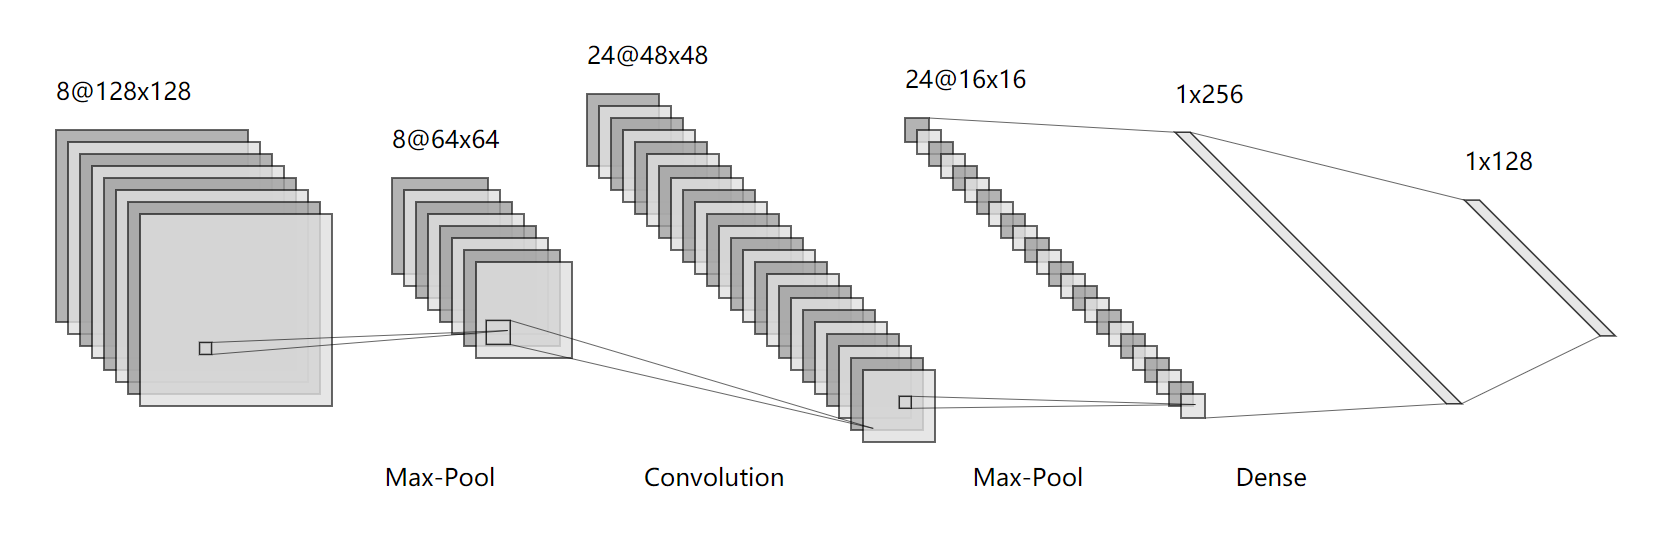
\includegraphics[width=12cm]{./figures/nn.png}
\caption{卷积神经网络实例}
\label{fig:nn}
\end{figure}

\section{卷积神经网络的理论}
\subsection{单层卷积层的神经网络}
\citet{du2018many}考虑了单层卷积层和单层平均池化层以及单层卷积层和单层全连接层组合的两种情况,\citet{du2018many}证明了两种情况下神经网络的均方误差的上下界。下面本文将对其结果进行总结和证明。
\subsubsection{单层卷积层加单层平均池化层}
对于输入$x\in \mathbb{R}^d$,考虑神经网络$F_1: \mathbb{R}^d \mapsto \mathbb{R}$,具体地,
\[
  F_1(x;w) = \sum_{l=0}^{r-1}w^{\top} \mathrm{P}_l^s x,
\]
其中$r\approx d/s$,$\mathrm{P}_l^s x=[x_{ls+1},x_{ls+2},\cdots,x_{ls+m}]$,神经网络的结构如图
\begin{figure}
\centering
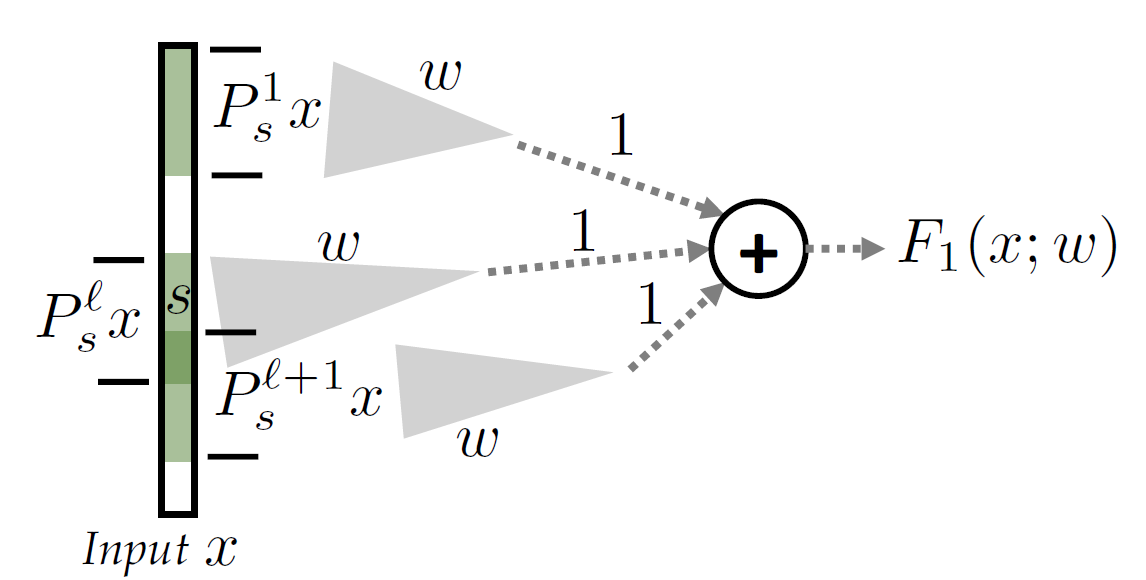
\includegraphics[width=10cm]{./figures/convp.PNG}
\caption{单层卷积层加单层平均池化层}
\label{fig:convp}
\end{figure}
\par
设$\{x_i,y_i\}_{i=1}^n$ 为$n$个训练样本数据,其中$x_i \in \mathbb{R}^d$为输入向量,而$y\in \mathbb{R}$为对应的值。由于实际的数据并不是完全由对应关系决定,而可能会加入噪声,所以这里引入均值为0的噪声,即
\[
  y_i = F_1(x_i;w_0)+\varepsilon_i,
\]
其中$\mathbb{E}[\varepsilon_i|x_i] = 0$,输入数据$\{x_i\}_{i=1}^n$从一个未知的分布$\mu$中独立同分布(i.i.d)的取样得到,并且$\mathrm{supp}\mu = \mathbb{R}^d$,即对于$\forall A \in \sigma(\mathbb{R}^d), \mu(A) > 0$,其中$\sigma(\cdot)$为$\sigma-$代数。
\par
对于数据的分布和噪声,有以下的假设:
\begin{assumption}[Sub-Guassian Noise]
存在一个有限常数$\sigma^2< \infty$,满足对$\forall t \in \mathbb{R}, \mathbb{E}[e^{t\varepsilon_i}] \leq e^{\sigma^2t^2/2}$
\end{assumption}
\begin{assumption}
存在一个有限常数$\nu^2< \infty$,满足对$\forall a \in \mathbb{R}^d, \mathbb{E}_\mu x = 0$,有$\mathbb{E}_\mu[\exp\{a^\top x\}]\leq \exp\{\nu^2\|a\|_2^2/2\}$
\end{assumption}
\begin{assumption}
存在正常数$\kappa > 0$,满足$\lambda_{\min}(\mathbb{E}_\mu x x^\top )\geq \kappa$
\end{assumption}
\par
这里的目标是通过训练数据训练神经网络的参数——权重$w$,即
\[
	arg\min_{\hat{w_n}} \sqrt{\mathbb{E}_{x\sim\mu}|F_1(x;\hat{w_n})- F_1(x;w_0)|^2}.
\]
\par
这里定义$\mathfrak{M}(n;F_1) = \inf_{\hat{w_n}}\sup_{w_0}\mathbb{E}_{\mu,w_0}[err(\hat{w_n},w_0)]$,其中$err(\hat{w_n},w_0) = \sqrt{\mathbb{E}_{x\sim\mu}|F_1(x;\hat{w_n})- F_1(x;w_0)|^2}$,则有以下的结果,它给出了$\mathfrak{M}(n;F_1)$的一个上界。
\begin{theorem}\label{theo:1}
对于$\delta\in (0,1/2)$和充分大的$n$,对于$\{x_i\}_{i=1}^n$的随机抽样,有$1-\delta$的概率,以下成立
\[
	\mathfrak{M}(n;F_1) \lesssim \sqrt{\frac{\sigma^2 m \log d}{n}},
\]
其中,$\lesssim$表示在不计常数下的$<$。
\end{theorem}
\par
定理~\ref{theo:1}~的证明过程见附录~\ref{pr:1}。

\par
根据定理~\ref{theo:1}~知,所给上界的收敛速率为$O(1/\sqrt{n})$,并且由上界的形式可以知道,所给上界与神经网络的大小没有关系。
\par
以上给出了$\mathfrak{M}$的一个上界,下面将给出其一个下界。
\begin{theorem}\label{theo:2}
假设输入数据$x_i$独立同分布于$\mathcal{N}\sim (0,I)$,假设$\varepsilon_i$独立同分布于$\mathcal{N}(0,\sigma^2)$,则存在一个固定常数$C > 0$满足
\begin{equation}
\mathfrak{M}(n,F_1) \geq C\sqrt{\frac{\sigma^2 m}{n}}
\end{equation}
\end{theorem}



\subsubsection{单层卷积层加单层全连接层}
对于单层卷积层加单层全连接层的神经网路,\citet{du2018many}给出了与单层卷积层单层平均池化层相类似的结果。
\par
对于输入$x\in \mathbb{R}^d$,考虑神经网络$F_2: \mathbb{R}^d \mapsto \mathbb{R}$,具体地,
\[
  F_1(x;w) = \sum_{l=0}^{r-1}a_l w^{\top} \mathrm{P}_l^s x,
\]
其中$r\approx d/s$,$\mathrm{P}_l^s x=[x_{ls+1},x_{ls+2},\cdots,x_{ls+m}]$,神经网络的结构如图
\begin{figure}
\centering
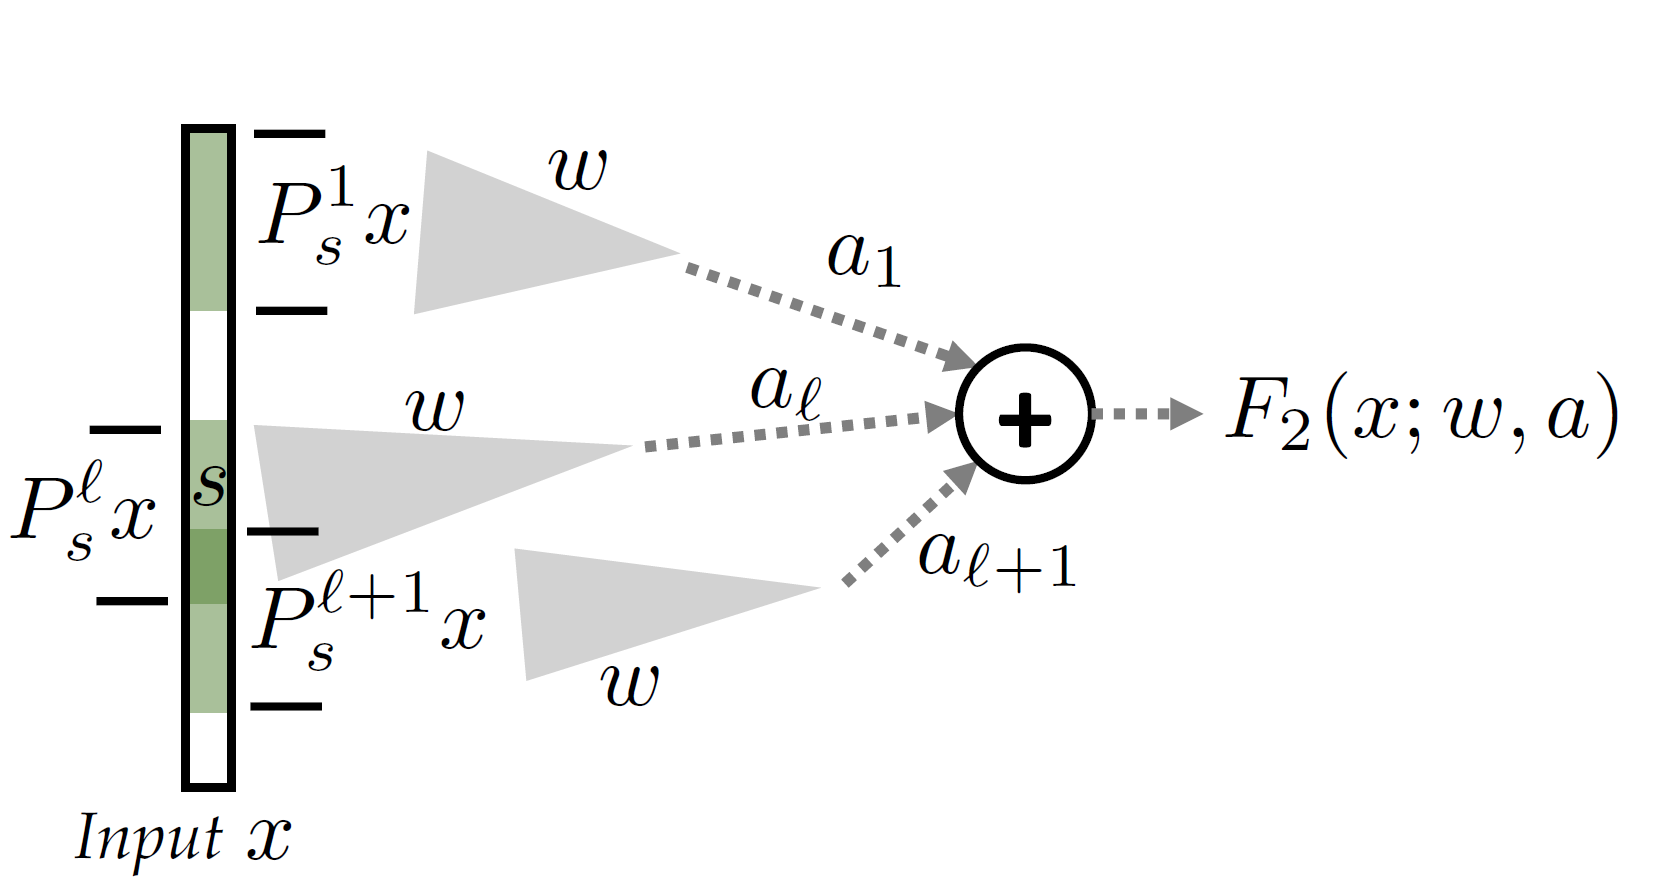
\includegraphics[width=10cm]{./figures/convf.PNG}
\caption{单层卷积层加单层全连接层}
\label{fig:convf}
\end{figure}
\par
设$\{x_i,y_i\}_{i=1}^n$ 为$n$个训练样本数据,在这里有
\[
  y_i = F_2(x_i;w_0)+\varepsilon_i.
\]
\par
对于数据的分布和噪声的假设与前一部分一样。
\par
这里定义$\mathfrak{M}(n;F_1) = \inf_{\hat{w_n}}\sup_{w_0}\mathbb{E}_{\mu,w_0}[err(\hat{w_n},w_0)]$,其中$err(\hat{w_n},w_0) = \sqrt{\mathbb{E}_{x\sim\mu}|F_2(x;\hat{w_n})- F_2(x;w_0)|^2}$,则有以下的结果,它给出了$\mathfrak{M}(n;F_2)$的一个上界。
\begin{theorem}\label{theo:3}
对于$\delta\in (0,1/2)$和充分大的$n$,对于$\{x_i\}_{i=1}^n$的随机抽样,有$1-\delta$的概率,以下成立
\[
	\mathfrak{M}(n;F_2) \lesssim \sqrt{\frac{\sigma^2 \min\{d,m+(d/s)\times (m/s)\}\cdot \log d}{n}},
\]
其中,$\lesssim$表示在不计常数下的$<$。
\end{theorem}


\par
根据定理~\ref{theo:3}~知,所给上界的收敛速率为$O(1/\sqrt{n})$,并且由上界的形式可以知道,所给上界与神经网络的大小没有关系。
\par
以上给出了$\mathfrak{M}$的一个上界,下面将给出其一个下界。
\begin{theorem}\label{theo:4}
假设输入数据$x_i$独立同分布于$\mathcal{N}\sim (0,I)$,假设$\varepsilon_i$独立同分布于$\mathcal{N}(0,\sigma^2)$,则存在一个固定常数$C > 0$满足
\begin{equation}
\mathfrak{M}(n,F_2) \geq C\sqrt{\frac{\sigma^2 (m+d/s)}{n}}
\end{equation}
\end{theorem}



\subsection{多层卷积神经网络}
\citet{zhou2018understanding}走的比\citet{du2018many}更远一步,他们考虑了多层卷积神经网络的优化能力和泛化能力,给出了理论的界。下面本文将对其结果进行介绍。
\subsubsection{记号及基本假设}
这里考虑一个$L$层卷积层的卷积神经网络$f(w;X)$,其中$w\in \mathbb{R}^d$为网络的参数,输入数据为$X\in \mathbb{R}^{r_0\times c_0}$,网络的输出为$v\in \mathbb{R}^{d_{l+1}}$,第$i$层卷积层的输入为$X_{i-1} \in \mathbb{R}^{\tilde{r}_{i-1}\times \tilde{c}_{i-1}\times \tilde{d}_{i-1}}$,输出为$X_{i} \in \mathbb{R}^{\tilde{r}_{i}\times \tilde{c}_{i}\times \tilde{d}_{i}}$。第$i$层卷积层进行的计算如下:
\[
 Z_i(:,:,j) = X_{i-1}\circledast W_i^j \in \mathbb{R}^{r_i\times c_i}, \forall j=1,\cdots,d_i,
\]
\[
Y_i = \sigma_1(Z_i)\in \mathbb{R}^{r_i\times c_i \times d_i},
\]
\[
 X_i = pool(Y_i) \in \mathbb{R}^{\tilde{r}_i\times \tilde{c}_i \times d_i},
\]
其中,$W_i^j \in \mathbb{R}^{k_i\times k_i \times d_{i-1}}$为第$i$个卷积层的第$j$个卷积核,$\circledast, pool(\cdot), \sigma_1(\cdot)$分别代表卷积操作、池化和sigmoid函数。
\par
整个网络的最后一层为一个全连接层,则最后一层的计算为
\[
u = W_{l+1}x_i \in \mathbb{R}^{d_{l+1}},
\]
\[
v = \sigma_2(u) \in \mathbb{R}^{d_{l+1}},
\]
其中,$x_i = vec(X_i)$为$X_i$的向量化,$\sigma_2(\cdot)$为softmax函数。
\par
这里我们考虑的损失函数为
\[
	\tilde{Q}_n(w) = \frac{1}{n} l(f(w;X_i), y_i),
\]
其中$l(f(w;X),y) = \frac{1}{2}\|v-y\|_2^2$,同时,模型在整体分布上的误差为
\[
	Q(w) = \mathbb{E}_{X,y \sim \mathcal{D}} l(f(w;X),y),
\]
其中$\mathcal{D}$为输入数据的分布。
\par
为了证明$\tilde{Q}_n(w)$可以收敛到$Q(w)$,这里需要先引入两个基本假设。
\par
第一条假设神经网络的权重为有界的。
\begin{assumption}
第$i$层卷积层的第$j$个卷积核$W_i^j\in\mathbb{R}^{k_i\times k_i \times d_{i-1}}$和$W_{L+1}\in \mathbb{R}^{d_{L+1}\times \tilde{r_L}\tilde{c_L}d_L}$均有界
\[
\|W_i^j\|_F \leq b_i (1\leq j\leq d_i; 1\leq i \leq L ),
\]
\[
\|W_{L+1}\|_F \leq b_{L+1},
\]
其中$b_i, 1\leq i \leq L+1$为有限正常数。
\end{assumption}
\par
这里,$\|\cdot\|_F$为Frobenius范数。
\par
在训练神经网络之后得到的参数往往都是非满秩的,所以作以下的假设
\begin{assumption}
设$\tilde{W}_i = [vec(W_i^1), vec(W_i^2),\cdots, vec(W_i^{d_i})]$,则假设$rank(\tilde{W}_i) \leq a_i, rank(W_{L+1}\leq a_{L+1})$.
\end{assumption}

\subsubsection{理论结果}
\par
基于以上的两个假设,有以下的结果
\begin{lemma}
在以上两个假设成立的条件下,如果$n\geq c_{f^\prime}L^2(b_{L+1}+\sum_{i=1}^L d_i b_i)^2 \max_i \sqrt{r_ic_i}/(\theta \varrho \epsilon^2)$,其中$c_{f^\prime}$为一个常数,则以概率$1-\epsilon$,有
\begin{equation}
\sup_{w\in \Omega} |\tilde{Q}_n(w)-Q(w)|\leq \sqrt{\frac{\theta \varrho +\log(4/\epsilon)}{2n}},
\end{equation}
其中$\theta = a_{L+1}(d_{L+1}+\tilde{r}_L\tilde{c}_Ld_L+1)+\sum_{i=1}^L a_i(k_i^2d_{i-1}+d_i+1),  \varrho = \sum_{i=1}^L \log\big(\frac{\sqrt{d_i}b_i(k_i-s_i+1)}{4p}\big)+\log(b_{L+1}) + \log{\frac{n}{128p^2}}$
\end{lemma}
\par
基于以上的引理,有以下的结果
\begin{theorem}\label{theo:2:1}
以概率$1-\epsilon$有
\[
\mathbb{E}_{(X,y)\sim \mathcal{D}}|\mathbb{E}_{\mathcal{A}}(Q(\tilde{w}) - \tilde{Q}_n(\tilde(w)))| \leq \sqrt{\frac{\theta \varrho + \log(4/\epsilon)}{2n}}
\]
\end{theorem}

\par
定理~\ref{theo:2:1}~说明了泛化误差的下降速度为$O(1/\sqrt{n})$。由于$\theta$代表了神经网络参数集的自由度数,它与神经网络的大小有关,为了降低泛化误差,需要有更多的训练数据。对于参数$\varrho$,其中的参数$k_1,s_i$都对神经网络的泛化误差有影响。$k_i$越大,则网络中的参数越多,训练网络更加困难,使得模型的泛化误差较大;而$s_i$越大,则网络的复杂度越低,训练越容易,模型的泛化误差越小。同时,$\theta, \varrho$中都含有$d_i$,这使得越宽的网络需要越多的训练数据进行训练,因为$d_i$越大,网络的参数越多,从而$\theta$增大。

\par
在给出泛化误差的控制之后,进一步考察模型是否可以达到训练过程的收敛,以下将分几步说明。

\begin{theorem}\label{theo:2:2}
在假设成立的情形下,经验梯度一致收敛,即,存在常数$c_{g^\prime}, c_g$,满足当$n \geq c_{g^\prime}\frac{L^2 b_{L+1}^2(b_{L+1}+\sum_{i=1}^Ld_ib_i)^2(r_0d_0c_0)^4}{d_0^4b_1^8(d\log(6)+\theta\varrho)\epsilon^2\max_i(r_ic_i)}$时,有
\[
\sup_{w\in \Omega} \|\nabla_w \tilde{Q}_n(w)-\nabla_wQ(w)\|_2\leq c_g \beta \sqrt{\frac{2d+\theta\varrho+\log(4/\epsilon)}{2n}}.
\]
\par
至少以概率$1-\epsilon$成立,其中
\[
\beta = [\frac{r_Lc_Ld_L}{8p^2}+\sum_{i=1}^L\frac{b_{L+1}^2d_{i-1}}{8p^2b_i^2d_i}r_{i-1}c_{i-1}\Pi_{j=i}^l\frac{d_jb_j^2(k_j-s_j+1)^2}{16p^2}]^{1/2},
\]
\[
d = \tilde{r}_L\tilde{c}_L d_Ld_{L+1}+\sum_{i=1}^L k_i^2d_{i-1}d_i.
\]
\end{theorem}
\par
从以上定理可见,经验梯度以$O(1/\sqrt{n})$收敛。下面的一个推论说明了$\nabla \tilde{Q}$和$\nabla Q_n$之间的关系。
\begin{corollary}\label{coro:2:1}
设定理~\ref{theo:2:2}~成立,并且$n \geq (d\varrho +\log(4/epsilon))\beta^2\epsilon$。则若由最小化经验误差得到的$\tilde{w}$使得$\|\nabla \tilde{Q}_n(\tilde{w})\|_2^2 \leq \epsilon$,则有$\|\nabla Q(\tilde{w})\|_2^2 \leq 4\epsilon$以至少概率$1-\epsilon$成立。
\end{corollary}
\par
推论~\ref{coro:2:1}~说明$\min \tilde{Q}_n$对应的最优解$\tilde{w}$和$\min Q$对应的最优解$w^*$十分接近,这说明了神经网络的有效性。
\par
为了更加准确的说明两者之间的关系,下面进一步考察驻点之间的差距。
\par
首先引入非退化驻点的概念。
\begin{definition}
驻点$w$称为非退化驻点,若
\[
\inf_i |\lambda_i(\nabla^2 Q(w))| \geq \xi ,
\]
其中$\xi$为一个正常数,$\lambda_i(\nabla^2 Q(w))$为Hessian矩阵$\nabla^2 Q(w)$的第$i$个特征值。
\par
驻点$w$称为鞍点,若$\nabla^2 Q(w)$的最小的特征值为负。
\end{definition}
\par
当$Q(w)$有一个非退化的驻点时,有以下结果。
\begin{theorem}\label{theo:2:3}
当$n \geq c_h \max(\frac{d+\theta\varrho}{\xi^2},\frac{L^2b_{L+1}^2(b_{L+1}+\sum_{i=1}^Ld_ib_i)^2(r_0c_0d_0)^4}{d_0^4 b_1^8d\varrho \epsilon^2\max_i(r_ic_i)})$,其中$c_h$为一常数。对$k\in\{1.\cdots,m\}$,存在$\tilde{Q}_n(w)$的非退化驻点$w_n^k$以至少概率$1-\epsilon$与$Q(w)$的非退化驻点$w_k$唯一地对应,同时,至少以概率$1-\epsilon$有
\[
\|w_n^k - w_k\|_2 \leq \frac{2c_g \beta}{\xi}\sqrt{\frac{2d+\theta\varrho+\log(4/\epsilon)}{2n}}\quad 1\leq k \leq m.
\]

\end{theorem}

\par
定理~\ref{theo:2:3}~说明,当训练样本的数量足够大时,$w_n^k$与$w_k$存在一一对应,并且二者之间的距离被$O(1/\sqrt{n})$控制住。对于退化驻点,由于Hessian矩阵的特征值中有0,使得它们之间没有一一对应。

\par
现在考虑另一类损失函数,具体的,设$l:\mathbb{R}\times \mathbb{R} \rightarrow [0,1]$是满足对所有的$y, l(\cdot,y)$为$\lambda-$Lipschitz的。输入数据为$x \in \mathbb{R}^{d\times d \times c}$,卷积层的卷积核为$K^i \in \mathbb{R}^{k\times k \times c\times c}, i\in\{1,\cdots,L\}$,卷积核的初始值为$K_0^i$,设$op(K^i)$为$K^i$的算子矩阵\cite{sedghi2018singular},且$\|op(K^i_0)\|_2 = 1$,定义卷积核与初始值之间的距离为$\|K-K_0\|_\sigma = \sum_{i=1}^L\|op(K^i) - op(K_0^i)\|_2$,定义$F_\beta = \{f_K : \|K-K_0\|+\sigma \leq \beta\}$,则有以下的结果,结果属于\citet{long2019size}。

\begin{theorem}
对任意的$\eta > 0$,存在$C>0$使得对任意$\beta, \delta > 0, \lambda \geq 1$,以及任意的$\mathbb{R}^{d\times d \times c}\times \mathbb{R}$的乘积$\sigma-$代数上的联合概率分布测度$P$,$\{(x_i, y_i)\}_{i=1}^n$独立同分布于$P$,则对$\forall f\in F_\beta$以至少概率$1-\delta$有
\[
\mathbb{E}_{z\sim P}[l_f(x,y)] \leq (1+\eta)\mathbb{E}_S [l_f] + \frac{C(Lk^2c^2(\beta+\log(\lambda n)) + \log(1/\delta))}{n}.
\]
\par
并且,$\beta \geq 5$时,有
\[
\mathbb{E}_{z\sim P}[l_f(x,y)] \leq \mathbb{E}_S[l_f]+C\sqrt{\frac{Lk^2c^2(\beta + \log(\lambda))+\log(1/\delta)}{n}}.
\]
\par
当$\beta < 5$时,有
\[
\mathbb{E}_{z\sim P}[l_f(z)] \leq \mathbb{E}_S[l_f]+ C\big(\beta \lambda \sqrt{Lk^2c^2/n} + \sqrt{\frac{\log(1/\delta)}{n}}\big),
\]
其中$l_f(x,y) = l(f(x),y)$
\end{theorem}

\par
上述定理给出了对CNN的泛化能力的一个估计,利用训练误差控制住了CNN在测试集上的误差。



%%% 其它部分
\backmatter

%% 本科生要这几个索引,研究生不要。选择性留下。
% 插图索引
\listoffigures
% 表格索引
\listoftables
% 公式索引
\listofequations


%% 参考文献
% 注意:至少需要引用一篇参考文献,否则下面两行可能引起编译错误。
% 如果不需要参考文献,请将下面两行删除或注释掉。
\bibliographystyle{thuthesis-numeric}      % 顺序编码制
% \bibliographystyle{thuthesis-author-year}  % 著者-出版年制
% \bibliographystyle{thuthesis-bachelor}     % 本科生参考文献的著录格式
\bibliography{ref/refs}


%%谢
% 如果使用声明扫描页,将可选参数指定为扫描后的 PDF 文件名,例如:
% \begin{acknowledgement}[scan-statement.pdf]
\begin{acknowledgement}
  衷心感谢导师 xxx 教授和物理系 xxx 副教授对本人的精心指导。他们的言传身教将使
  我终生受益。

  在美国麻省理工学院化学系进行九个月的合作研究期间,承蒙 xxx 教授热心指导与帮助,不
  胜感激。感谢 xx 实验室主任 xx 教授,以及实验室全体老师和同学们的热情帮助和支
  持!本课题承蒙国家自然科学基金资助,特此致谢。

  感谢 \LaTeX 和 \thuthesis\cite{thuthesis},帮我节省了不少时间。
\end{acknowledgement}


%% 附录
\begin{appendix}
\chapter{外文资料的调研阅读报告或书面翻译}

\title{在结构化数据上用随机梯度下降算法学习过参数化神经网络\cite{li2018learning}}

{\heiti 摘要:} 神经网络有许多成功的应用,而理论上的理解却少得多。为了弥补这一缺陷,我们研究了从随机初始化中通过随机梯度下降(SGD)学习用于多类分类的双层超参数ReLU神经网络的问题。在过参数化的情况下,当数据来自分离良好的分布时,我们证明了SGD学习的网络具有较小泛化误差,尽管该网络具有足够的能力来适应任意标签。此外,该分析对学习神经网络的几个方面提供了有趣的见解,并可通过对合成数据和MNIST数据集的实验加以验证。

\section{背景介绍}
神经网络在许多应用中取得了巨大的成功,但尽管最近理论研究有所增加,但仍有许多问题有待解释。例如,根据经验观察,在过参数化设置(即,需要学习的参数数量大于训练数据点数量的大型网络)中使用随机梯度下降(SGD)进行学习不会导致过度拟合[24,31]。一些最近的研究使用低复杂度的学习算法来解释泛化,但通常不能解释SGD或其变体如何支持低复杂度的算法(即,归纳偏差或隐式正则化)[3, 23]。我们还观察到,过参数化和适当的随机初始化有助于优化[28、12、26、18],但也不清楚为什么特定的初始化可以改善学习过程。此外,大部分试图解释这些现象的现有作品依赖于关于数据分布的不切实际的假设,例如高斯性和/或线性可分性〔32, 25, 10,17, 7〕。
\par
因此,本文提出在更真实的数据结构上,研究利用SGD进行分类的两层超参数神经网络的学习问题。特别是,每个类中的数据是几个元素的混合,不同类的元素在距离上有很好的分隔(但是每个类中的元素可以彼此接近)。这是由实际数据驱动的。例如,在数据集MNIST[15]上,每个类对应于一个数字,并且可以具有对应于数字的不同写入样式的多个元素,其中的图像是其中一个元素的小扰动。另一方面,属于同一分量的图像比另一个数字的图像更接近彼此。在此设置中进行分析可以帮助理解实际数据的结构如何影响优化和泛化。
\par
在这种情况下,我们证明了当网络充分过参数化时,可证明SGD可以学习到接近随机初始化且具有小的泛化误差的网络。结果表明,在过参数化的情况下,当数据结构良好时,虽然原则上网络可以过拟合,但随机初始化的SGD引入了很强的归纳偏差,具有很好的泛化能力。
\par
我们的结果还表明,过参数化要求和学习时间取决于数据结构固有的参数,而不是数据的环境维度。更重要的是,通过分析得到的结果也为神经网络学习的各个方面提供了一些有趣的理论见解。它揭示了学习的成功关键依赖于过参数化和随机初始化。这两者结合在一起,导致SGD和另一个具有良性优化环境的学习过程之间的初始化紧密耦合。这种耦合,加上数据的结构,使得SGD能够找到一个具有低泛化误差的解,同时仍然保持在上述初始化的领域内。我们的工作进一步解释了过参数化和随机初始化如何帮助优化,以及结构化数据上的SGD动力学上如何产生归纳偏差和良好的泛化。我们将在稍后的章节中讨论一些其他的技术内含,如在初始化时存在一个好的解,以及学习的权重的低秩性。对综合数据和基准数据集MNIST的补充实证研究为分析和见解提供了积极支持。

\section{相关工作}
\textbf{神经网络的泛化}。实验显示了神经网络泛化的一些有趣现象:实际的神经网络具有拟合随机标签的训练数据的能力,但在训练实际数据时仍具有良好的泛化能力[24,31,2]。由于这些网络的参数比统计上所需的参数多,因此它们是过参数化,而单纯地应用传统理论无法解释其良好的泛化性。多方面的工作提出了一些低复杂度的学习网络和衍生的泛化界限,以更好地解释。[3,23,21]证明了基于谱归一化裕度的泛化界,[9,23]从PAC-Bayes方法导出了界,以及[1,33,4]用压缩方法导出了界。一般来说,他们没有解决为什么会出现低复杂度。本文朝着这个方向迈出了一步,尽管是在两层网络和简化的数据模型上。
\par
\textbf{超参数化和隐式正则化}。过参数化网络的训练目标在原理上具有许多(近似)全局最优解,并且一些推广优于其他14, 8, 2种,而经验观察意味着实践中的优化过程更倾向于那些具有更好泛化性的网络。因此,一个有趣的问题是,这种隐式正则化或归纳偏差是如何从数据的优化和结构中产生的。最近的研究是针对不同任务的SGD,如logistic回归[27]和矩阵分解[11,19,16]。与我们的工作更相关的是[7],它研究了在线性可分数据上学习两层超参数网络的问题,并证明了SGD收敛到全局最优,具有很好的推广性。我们的工作研究了具有良好聚类(并且可能不是线性可分)结构的数据的问题,我们认为这种结构更接近实际情况,因此可以推进这一研究路线。
\par
学习神经网络的理论分析。还存在大量的工作,分析学习神经网络[13, 26, 30,10, 25, 29,6, 32, 17,5]的优化景观。一般来说,他们需要对数据假设不现实的假设,如高斯性,和/或对网络有很强的假设,如仅使用线性激活。他们也没有研究隐式正则化的优化算法。

\section{问题建模}
本文中,我们考虑一个两层的激活函数为ReLU的k-分类神经网络$f = (f_1,f_2,\cdots,f_k)$,满足对$\forall i \in [k]$,有
\[
f_i(x) = \sum_{r = 1}^m a_{i,r} ReLU(\langle w_r, x\rangle)
\]
其中$\{w_r\in \mathbb{R}^d\}$是隐藏层中的$m$个神经元的权重,$\{a_{i,r}\in \mathbb{R}\}$是最后一层的权重,$ReLU(z) = \max\{0,z\}$。
\par
\textbf{对数据的假设:}数据按照以下方式从分布$\mathcal{D}$中产生,一共有$k\times l$个$\mathbb{R}^d$上的未知分布$\{\mathcal{D}_{i,j}\}_{i\in [k] ,j \in [l]}$,和概率$p_{i,j}\geq 0$满足$\sum_{i,j}p_{i,j} = 1$。每个数据都是独立同分布地生成:(1) 取样$z\in [k]\times [l]$满足$Pr[z = (i,j)] = p_{i,j}$;(2) 设置标签$y = z[0]$,从分布$\mathcal{D}_z$中取样$x$。假设我们取了$n$个样$\{(x_i,y_i)\}_{i=1}^n$。
\par
让我们定义密度$\rho$在$\mathbb{R}^d$的分布$\mathcal{D}$的支撑集为$supp(D) = \{x:p(x)>0\}$,两个集$S_1,S_2\subset \mathbb{R}^d$之间的距离为$dist(S_1,S_2)= \min_{x\in S_1,y\in S_2}\{\|x–-y\|_2\}$,集$S_1\subset \mathbb{R}^d$的直径为$diam(S_1) = \max_{x,y\in S_1}\{\|x-y\|_2\}$。然后我们准备对数据进行假设。
\begin{itemize}
  \item[\textbf{A1}] (可分离性)存在$\delta >0$满足对任意的$i_1\neq i_2\in[k]$和任意的$j_1,j_2\in[l]$,$dist(supp(\mathcal{D}_{i_1,j_1}), supp(\mathcal{D}_{i_2,j_2}))\geq \delta$。除此之外,对任意的$i\in [k],j\in [l]$,$diam(supp(\mathcal{D}_{i,j}))\leq \lambda \delta$,其中$\lambda \leq 1/(8l)$。
  \item[\textbf{A2}] (正则性)对任意的$x$有$\|x\|_2 = 1$。
\end{itemize}
\par
有一些重要的记述。我们考虑的不是一个类只有一个分布,而是在每个类中有一个任意的$(l\geq 1)$分布,我们认为这更吻合实际数据。例如,在MNIST中,一个类可以是数字1,而l可以是不同的书写风格1(1或|或/)。
\par
假设(A2)是为了简单起见,而(A1)是我们的关键假设。当每个类中有$l \geq 1$分布时,我们的假设数据是不可线性分离的,例如$\mathbb{R}^d$中有两个类的异或型数据,一个类由两个直径为1/10的球组成,球的中心为(0,0)和(2,2),另一个类由两个直径相同的球组成,球的中心为(0,2)和(2,0)。有关说明请参见附录C中的图3。此外,我们这里唯一的假设是$\lambda = O(1/l)$。当$l=1$时,$\lambda = O(1)$,这是分布可被有效学习对$\lambda$的阶的最小要求。我们的工作允许更大的$l$,因此每个类中的数据可能更复杂。在这种情况下,我们对数据的可分离性的要求也更高。当我们增加$l$来细化每个类内的分布时,每个分布的直径应该也变小。只要每个分布的直径递减率大于分布的总数,那么我们的假设就成立。
\par
\textbf{关于学习过程的假设。}我们将只学习权重$w_r$来简化分析。由于ReLU激活函数是正单调的,所以过参数化的影响仍然可以研究,并且在以前的工作中已经采用了类似的方法[7]。所以网络也可写为$y = f(x,w) = (f_1(x,w),\cdots,f_k(x,w))$,其中$w = (w_1,\cdots, w_r)$。
\par
我们假设学习过程的初始化为随机的:
\begin{itemize}
  \item[(A3)](随机初始化)$w_r^{(0)}\sim \mathcal{N}(0,\sigma^2I), a_{i,r} \sim \mathcal{N}(0,1)$,其中$\sigma = \frac{1}{\sqrt{m}}$.
\end{itemize}
\par
学习过程最小化softmax函数的交叉熵,定义为:
\[
L(w) = -\frac{1}{N}\sum_{s = 1}^N \log o_{y_s}(x_s,w)
\]
其中$o_y(x,w) = \frac{e^{f_y(x,w)}}{\sum_{i=1}^k e^{f_i(x,w)}}$
\par
记$L(w,x_s,y_s) = -\log o_{y_s}(x_s,w)$记为单点$(x_s,y_s)$的交叉熵。
\par
我们把一个批量大小为$B$,迭代次数$T=N/B$,学习率$\eta$的小批量SGD看作如下过程:将训练样本随机分为$T$个批量,每个批量为$B$,让$T$个批量中的样本指标为$B_t$,每次迭代时,更新次数为
\[
w_r^{(t+1)} = w_r^{(t)} -\eta\frac{1}{B}\sum_{s\in \mathcal{B}_t} \frac{\partial L(w^{(t)},x_s,y_s)}{\partial w_r^{(t)}}, \forall r \in [m]
\]
其中
\[
\frac{\partial L(w,x_s,y_s)}{\partial w_r} = \bigg(\sum_{i\neq y_s} a_{i,r}o_i(x_s,w)-\sum_{i\neq y_s} a_{y_s,r}o_i(x_s,w)\bigg)
\]


\section{主要结果}
为了简化记号,对于目标误差$\epsilon$,以大概率的意思是以概率$1-1/poly(1/\delta,k,l,m,1/\epsilon)$为足够大的多项式,$\tilde{O}$忽略了$poly(\log(1/\delta),\log k, \log l, \log m,\log (1/\epsilon))$的因子。
\begin{theorem}
假设满足(A1)(A2)(A3)。那么对于每一个$\epsilon > 0$,$M = poly(k,l,1/\delta,1/\epsilon)$,满足对任意的$m\geq M$,在进行小批量SGD之后,批量大小为$B=poly(k,l,1/\delta,1/\epsilon,\log m)$,学习率$\eta = \frac{1}{m\cdot poly(k,l,1/\delta,1/\epsilon,\log m)}, T = poly(k,l,1/\delta,1/\epsilon,\log m)$次迭代,以高概率:
\[
Pr_{x,y\sim \mathcal{D}}[\forall j \in [k], j\neq y, f_y(x,w^{(T)}) > f_j(x,w^{(T)})] \geq 1-\epsilon 
\]
\end{theorem}
\par
我们的定理意味着如果数据满足我们的假设,并且我们对网络进行了适当的参数化,那么我们只需要在$k,l,1/\delta$的多个样本中使用多项式就可以获得良好的预测误差。这种误差是在真实分布$\mathcal{D}$上直接测量的,而不仅仅是在用于训练该网络的输入数据上。我们的结果也是无维度的:没有依赖于数据的基础维度$\mathcal{D}$,复杂性完全被$k,l,1/\delta$所俘获。此外,不管网络被过度参数化,它只会增加$\log m$的因子的总迭代,因此我们可以通过子指数量过参数化而不显著增加复杂性。
\par
此外,我们可以将每个输入示例视为单个分布,因此$\lambda$始终为零。在这种情况下,如果我们使用批处理大小$B$进行$T$迭代,那么我们将得到$l=N=BT$。然后我们的定理表明,只要$m=poly(N,1/\delta^\prime)$,其中$\delta^\prime$是每个示例之间的最小距离,我们实际上可以拟合输入数据的任意标签。然而,由于总迭代仅依赖于$\log m$,当$m=poly(N,1/\delta^\prime)$,但输入数据是实际结构化的($k,l$和$\delta$都很小)时,即使网络有足够的能力来适应训练示例的任意标签(SGD也可以这样做),SGD实际上也可以实现小的泛化误差。因此,我们证明了SGD对结构化数据具有很强的归纳偏向性:它没有找到一个适合任意标签的坏的全局最优解,而是找到那些具有良好泛化保证的全局最优解。这对[24,31]中的经验观察给出了更为彻底的解释。

\section{直观解释和简化情形的证明概要}
要训练具有ReLU激活的神经网络,需要解决两个问题:
\begin{enumerate}
\item 为什么SGD可以优化训练损失?或者找到一个临界点?由于下卧网络是高度非光滑的,现有定理没有给出任何具有Relu激活的神经网络的SGD的有限收敛速度。
\item 为什么经过训练的网络可以泛化?即使容量足够大,可以容纳输入数据的随机标签?这就是所谓的SGD的感应偏压。
\end{enumerate}
\par
这项工作朝着回答这两个问题迈出了一步。研究表明,当网络参数过高时,网络变得更为“伪光滑”,这使得SGD更容易将训练损失降到最小,而且不会对泛化误差造成影响。我们的证明基于以下重要观察:
\begin{itemize}
  \item 我们越是过度参数化网络,一个神经元和一个数据点的激活模式在固定次数的迭代中改变的可能性就越小。
\end{itemize}
\par
这个观察使我们能够将真实神经网络的梯度与“伪梯度”耦合起来,其中每个数据点和每个神经元的激活模式是固定的。也就是说,当计算“伪梯度”时,对于固定$R,i$,在第$i$个数据点席上是否激活第$R$个隐节点,对于不同的$T$,总是相同的(但对于固定的$T$,对于不同的$R$或$I$,符号可以是不同的)。我们可以证明,除非泛化误差小,否则“伪梯度”总是会出现。做大点。此外,我们还证明了该网络实际上是光滑的,因此SGD可以使损失最小化。
\par
然后我们证明,当隐神经元的数目$m$增加时,在适当降低学习率的情况下,使损失最小化所需的迭代总数基本不变。但是,我们可以将真实梯度与伪梯度耦合的迭代总数增加。因此,有一个多项式大$m$,这样我们可以耦合这两个梯度,直到网络达到一个小的泛化误差。

\subsection{一个简化情形:无方差}
在这里,我们演示了一个简化案例的证明草图,附录a提供了证明。一般情况的证明见附录B。在简化情况下,我们进一步假设:
\begin{itemize}
\item[\textbf{(S)}](无方差)每个$\mathcal{D}_{a,b}$是一个单独的数据点$(x_{a,b},a)$,而且我们正在做与小批量SGD相反的全批量梯度下降。
\end{itemize}

\par
我们重新记损失函数为$L(w) = \sum_{a\in[k],b\in[l]}p_{a,b} L(w,x_{a,b},a)$,且梯度为
\[
\frac{\partial L(w)}{\partial w_r} = \sum_{a\in[k], b\in [l]}p_{a,b}\bigg(\sum_{i\neq a}a_{i,r}o_i(x_{a,b},w) - \sum_{i\neq a} a_{a,r}o_i(x_{a,b},w)\bigg)\mathbb{I}\{\langle w_r, x_{a,b}\rangle \geq 0\}x_{a,b}
\]
\par
我们如下定义伪梯度:
\[
\frac{\tilde{\partial} L(w)}{\partial w_r} = \sum_{a\in[k], b\in [l]}p_{a,b}\bigg(\sum_{i\neq a}a_{i,r}o_i(x_{a,b},w) - \sum_{i\neq a} a_{a,r}o_i(x_{a,b},w)\bigg)\mathbb{I}\{\langle w_r^{(0)}, x_{a,b}\rangle \geq 0\}x_{a,b}
\]
其中我们用$\mathbb{I}\{\langle w_r^{(0)}, x_{a,b}\rangle \geq 0\}$代替真梯度中的$\mathbb{I}\{\langle w_r, x_{a,b}\rangle \geq 0\}$。即,激活状态由初始状态决定。直观上,伪梯度是一个伪网络$g$中的梯度(但是并不完全一样),定义为$g_i(x,w) = \sum_{r = 1}^m a_{i,r}\langle w_r, x\rangle \mathbb{I}\{\langle w_r^{(0)},x\rangle\geq 0\}$.
\par
耦合两个梯度则相当于耦合两个网络。
\par
为了简化,让$v_{a,a,b} = \sum_{i\neq a} o_i(x_{a,b},w) = \frac{\sum_{i\neq a} e^{f_i(x_{a,b},w)}}{\sum_{i=1}^k e^{f_i(x_{a,b},w)}}$,当$s\neq a,v_{s,a,b} = -o_s(x_{a,b},w) = -\frac{f_s(x_{a,b},w)}{\sum_{i=1}^k e^{f_i(x_{a,b},w)}}$。粗略地说,如果$v_{a,a,b}$小时,$f_a(x_{a,b},w)$相较于其他$f_i(x_{a,b},w)$来说较大,所以分类误差较小。
\par
我们证明了以下两个主要引理。第一种说法是,在每次迭代中,其梯度可以与伪梯度耦合的隐藏单元的总数是相当大的。

\begin{lemma}
初始化以大概率,当$\tau>0$,对任意的$t = \tilde{O}(\frac{\tau}{\eta})$,我们有对至少$1-\frac{e\tau kl}{\sigma}$比例的$r\in [m]: \frac{\partial L(w^{(t)})}{\partial w_r} = \frac{\tilde{\partial}L(w^{(t)})}{\partial w_r} $
\end{lemma}
\par
第二条引理说明伪梯度较大除非误差较小。
\begin{lemma}
对$m = \tilde{\Omega}(\frac{k^3 l^2}{\delta})$,对所有的$\{p_{a,b}v_{i,a,b}\}_{i,a\in[k],b\in[l]}\in[-v,v]$,满足$\max \{p_{a,b}v_{i,a,b}\}_{i,a\in[k],b\in[l]} = v$,存在至少$\Omega(\frac{\delta}{kl})$比例的$r\in[m]$满足$\|\frac{\tilde{\partial} L(w)}{\partial w_r}\|_2 = \tilde{\Omega}(\frac{v\delta}{kl})$
\end{lemma}
\par
现在我们展示利用这两个引理证明对一个足够小的学习率$\eta$算法可以收敛。为了简单起见,假设$kl/\delta = O(1),\epsilon = o(1)$。 因此通过引理5.2我们知道除非$v\leq \epsilon$,存在$\Omega(1)$比例的$r$满足$\|\tilde{\partial}L(w)/\partial w_r\|_2 = \Omega(\epsilon)$。除此之外,通过引理5.1我们之道可以选取$\tau = \Theta(\sigma\epsilon)$即$e\tau/\sigma = \Theta(\epsilon)$,这说明存在$\Omega(1)$比例的$r$满足$\|\tilde{\partial}L(w)/\partial w_r\|_2 = \Omega(\epsilon)$。对于足够小的学习率$\eta$,一步的梯度下降会使$L(w)$下降$\Omega(\eta m \epsilon^2)$,所以算法在$t = O(1/\eta m \epsilon^2)$次迭代后会收敛。最后我们只需说明$1/\eta m \epsilon^2\leq O(\tau/\eta) = \Theta(\sigma\epsilon/\eta)$,所以我们始终可以应用引理5.1。因为$\sigma = \tilde{O}(1/\sqrt{m})$,我们知道只要$m\geq poly(1/\epsilon)$。一个小的$v$可以使得泛化误差也很小。

\section{关于分析中的原理的讨论}
我们的分析虽然是为了在结构良好的数据上学习两层网络,但也为在更一般的环境下学习神经网络提供了一些启示。
\par
一般化。最近几行的工作解释了学习网络的低复杂度的泛化网络的泛化现象,从频谱归一化边缘[3, 23, 21]、压缩[1, 33, 4]和PAC Bayes[9, 23]的观点来看。
\par
我们的分析已经部分地解释了如何结构化数据上的SGD(适当的随机初始化)导致从压缩和PCA贝叶斯点视图的低复杂度。我们已经证明,在随机初始化的一个邻域中,w.h.p.梯度与另一个良性学习过程的梯度相似,因此SGD可以在仍然处于邻域中的情况下减小误差并获得一个好的解。接近初始化意味着权重(或者更准确地说,学习的权重和初始化之间的差异)可以很容易地压缩。事实上,在文献[22,1]中,我们已经进行了经验观察,并将其与泛化联系起来。此外,[1]使用helper字符串显式地指出了这种压缩(与我们设置中的初始化相对应)。[1] 同时指出压缩视图可以看作是PAC-Bayes视图的一种更为明确的形式,因此我们的直觉也适用于后者。
\par
在初始化过程中存在一个小的泛化误差的解决方案本身并不明显。直观地说,在结构化数据上,更新是分布在隐藏神经元权重上的结构化信号。然后对于预测,权值中的随机初始化部分具有很强的对消性,而权值中的结构化信号部分共同影响输出。因此,后者可以比前者小得多,而网络仍然可以给出准确的预测。换言之,在离初始化不远的地方可能有一个高概率的解决方案。

\par
对权重的低阶提供了一些见解。更确切地说,当数据被良好地聚集在几个模式周围时,累积的更新(学习权重和初始化之间的差值)应该是近似低秩的,这可以从检查SGD更新看出。然而,当与初始值相比差异很小时,最终权重矩阵的谱由初始值的谱支配,因此将趋向于更接近随机矩阵的谱。同样,这些观察/直觉已经在文献中提出,并且与压缩和泛化(例如,[1])相关。
\par
数据的隐式正则化v.s.结构。已有的工作已经分析了SGD在Logistic回归(27)、矩阵分解(11, 19, 16)和线性可分数据(7)上学习两层网络的隐式正则化。我们的设置和分析技术与现有的工作相比是新颖的。研究结构化数据的一个动机是理解结构化数据在隐式正则化中的作用,即观察到在较少结构化甚至随机数据上学习的解远离初始化。事实上,我们的分析表明,当网络大小是固定的(并且充分过参数化)时,对结构较差的数据(较大的K和‘)的学习需要更多的迭代,因此该解决方案可以更多地偏离初始化,并且具有更高的复杂性。一个极端且特别有趣的情况是,当网络被过度参数化时,原则上它可以通过将每个点视为一个组件来拟合训练数据,而实际上它们来自具有少量组件的结构化分布。在这种情况下,我们可以证明它仍然学习一个具有小泛化误差的网络;请参阅第4节中的更多技术讨论。
\par
我们还注意到,我们的分析是在假设网络有足够多的内存的情况下进行的,即m是k的一个足够大的多项式,以及测量数据结构的其他相关参数。可能存在m小于此多项式但足以拟合数据的情况,即网络仍然是过度参数化的。尽管在这种情况下,分析仍然提供了有用的见解,但它并没有完全适用;另一方面,我们用相对较小的m进行了实验。经验观察[24,31]表明,实际的网络高度参数化,因此我们的直觉可能仍然有帮助。
\par
随机初始化的影响。我们的分析也显示了适当的随机初始化如何有助于优化,从而推广。本质上,这保证了对于接近初始化的权重,许多隐藏的ReLU单元将具有与初始化相同的激活模式(即,激活与否),这意味着邻域中的梯度类似于隐藏单元具有固定激活模式时的梯度。这使得SGD在损失较大时取得进展,并最终获得一个好的解决方案。我们还注意到,必须仔细设置初始化的规模,这是一个广泛研究的主题[20,28]。我们的初始化有一个与隐藏单元数量相关的比例,这在网络大小变化时特别有用,因此可以在这种实际设置中引起兴趣。

\begin{figure}
\centering
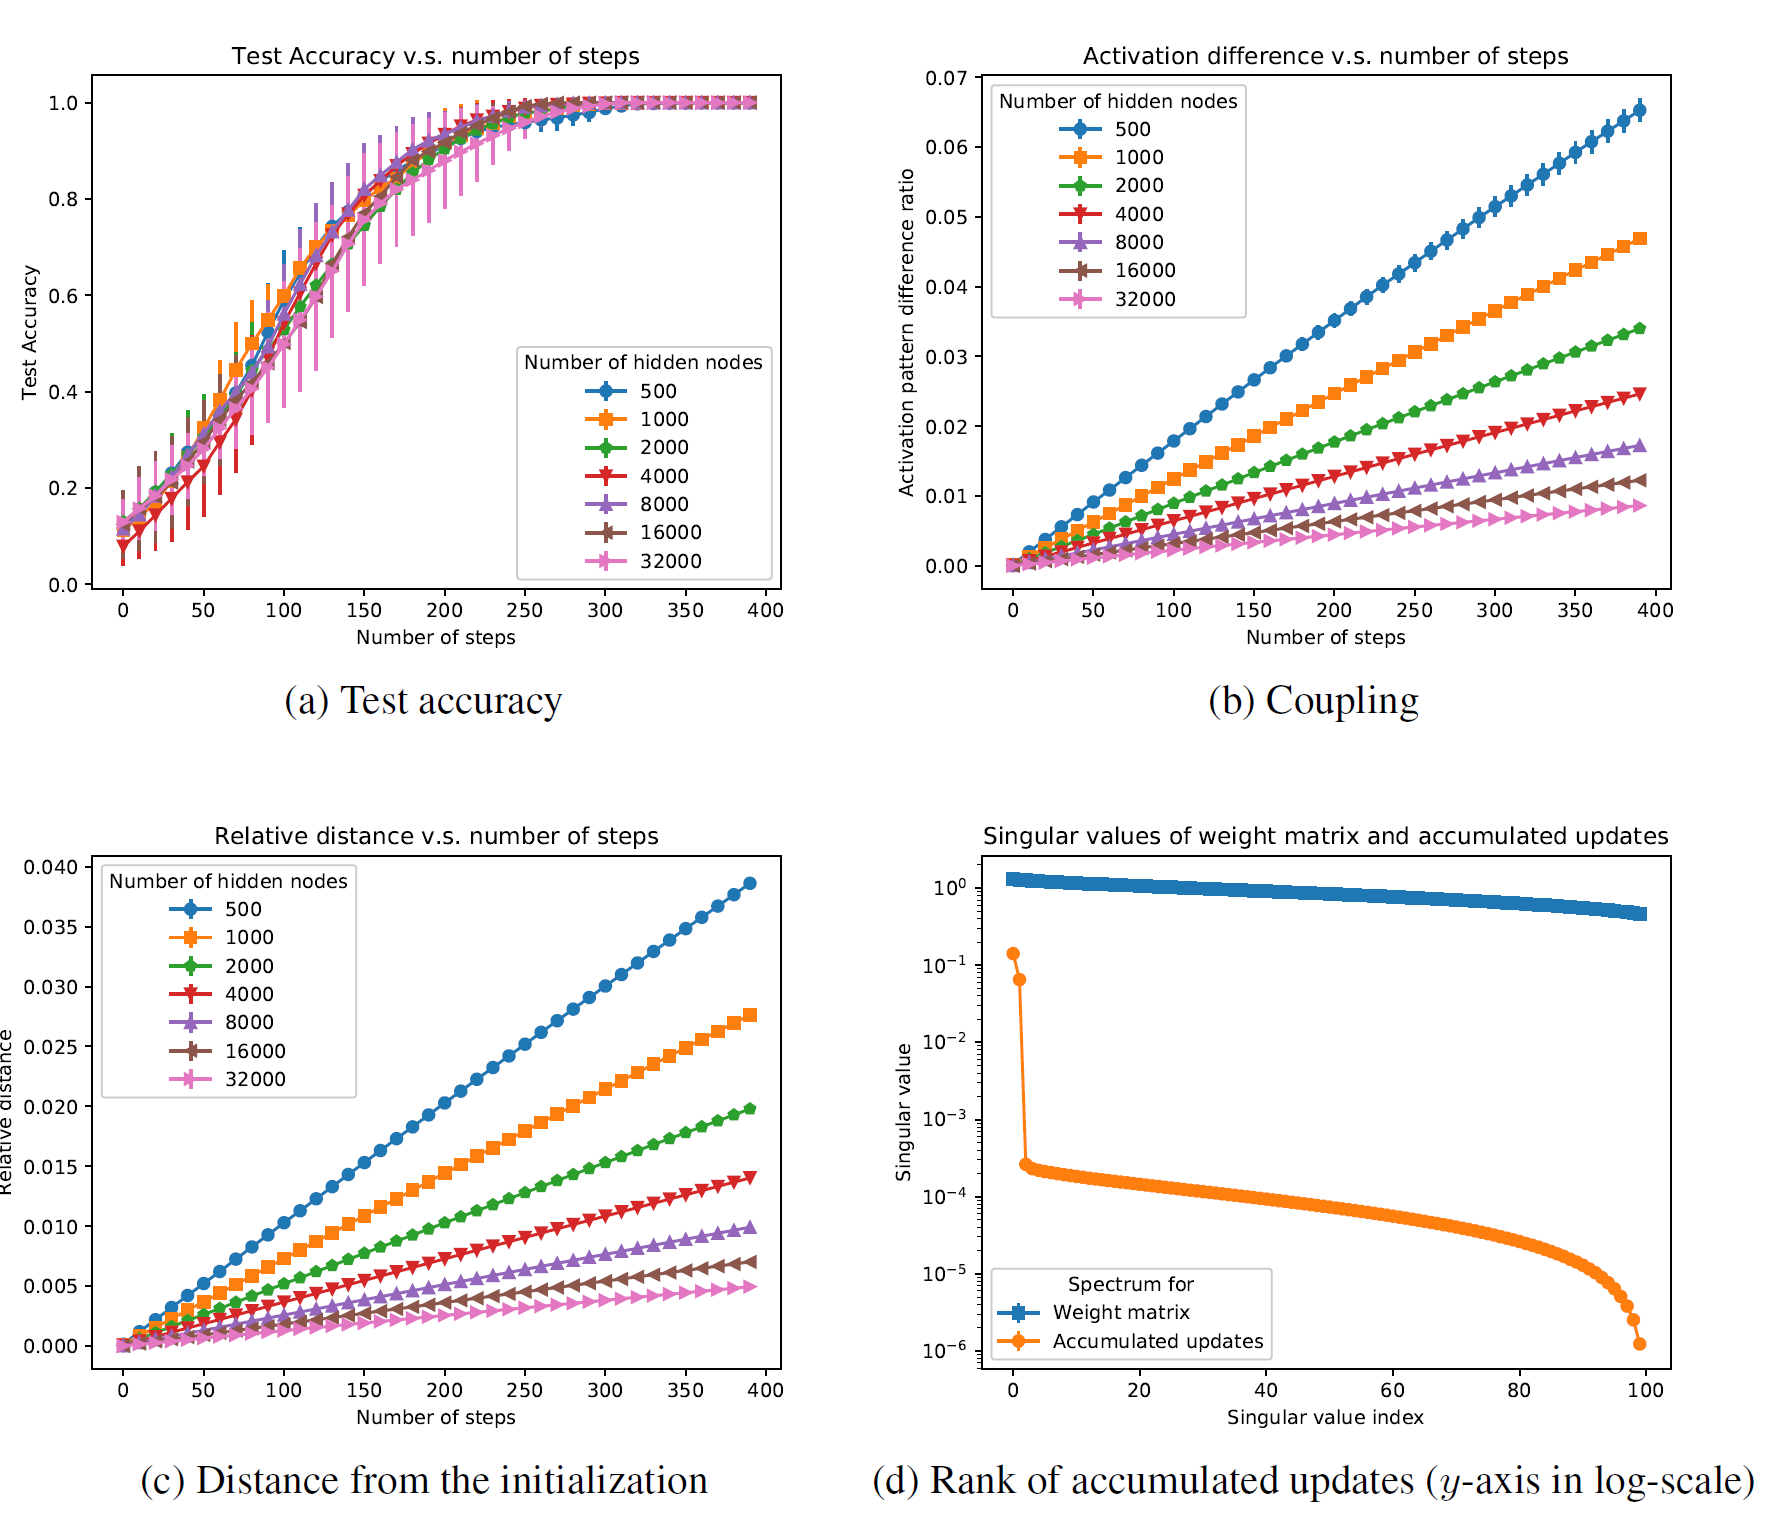
\includegraphics[width=12cm]{./figures/results.png}
\caption{在合成数据上的结果}
\end{figure}


\section{实验}
本节旨在验证一些关键含义:(1)隐藏单元的激活模式与初始化时的激活模式耦合;(2)与初始化的大小相比,从初始化到学习的解的距离相对较小;(3)累积的更新(即学习的权重矩阵之间的差异和初始化)具有近似低秩。合成数据和MNIST数据的结果确实支持这一点。附加实验见附录D。
\par
设置。合成数据是1000维的,由$k=10$个类组成,每个类都有$l=2$个分量。每个分量的概率均为$1/kl$,是协方差为$\sigma^2 / dI$的高斯分布,其平均值为从高斯分布$\mathcal{N}(0,\sigma^2_0 d)$中采样的i.i.d.,其中$\sigma = 1$和$\sigma_0 = 5$。抽取1000个训练数据点和1000个测试数据点。
\par
网络结构和学习过程遵循第3节;实验中隐藏单元$m$的个数变化,权值初始为$\mathcal{N}(0,1/m)$。在综合数据上,SGD运行为$T=400$步,批大小$B=16$,学习率$\eta = 10/m$。在MNIST上,SGD运行为$T=2×104$步,批大小$B=64$,学习率$\eta=4×103/m$。
\par
除了测试精度外,我们还报告了三个对应于待验证的三个观测/影响的量。首先,对于耦合,我们计算其激活模式与初始化时相比发生变化的隐藏单元的分数。这里,如果ReLU的输入为正,激活模式定义为1,否则定义为0。其次,对于距离,我们计算相对比率$\|w^{(t)} - w^{(0)}\|_F/\|w^{(0)}\|_F$,其中$w^{(t)}$是时间$t$时的权重矩阵。最后,对于累积更新的秩,我们绘制$w^{(T)}-w^{(0)}$的奇异值,其中$T$是最后一步。所有实验重复5次,并报告平均值和标准偏差。

\begin{figure}
\centering
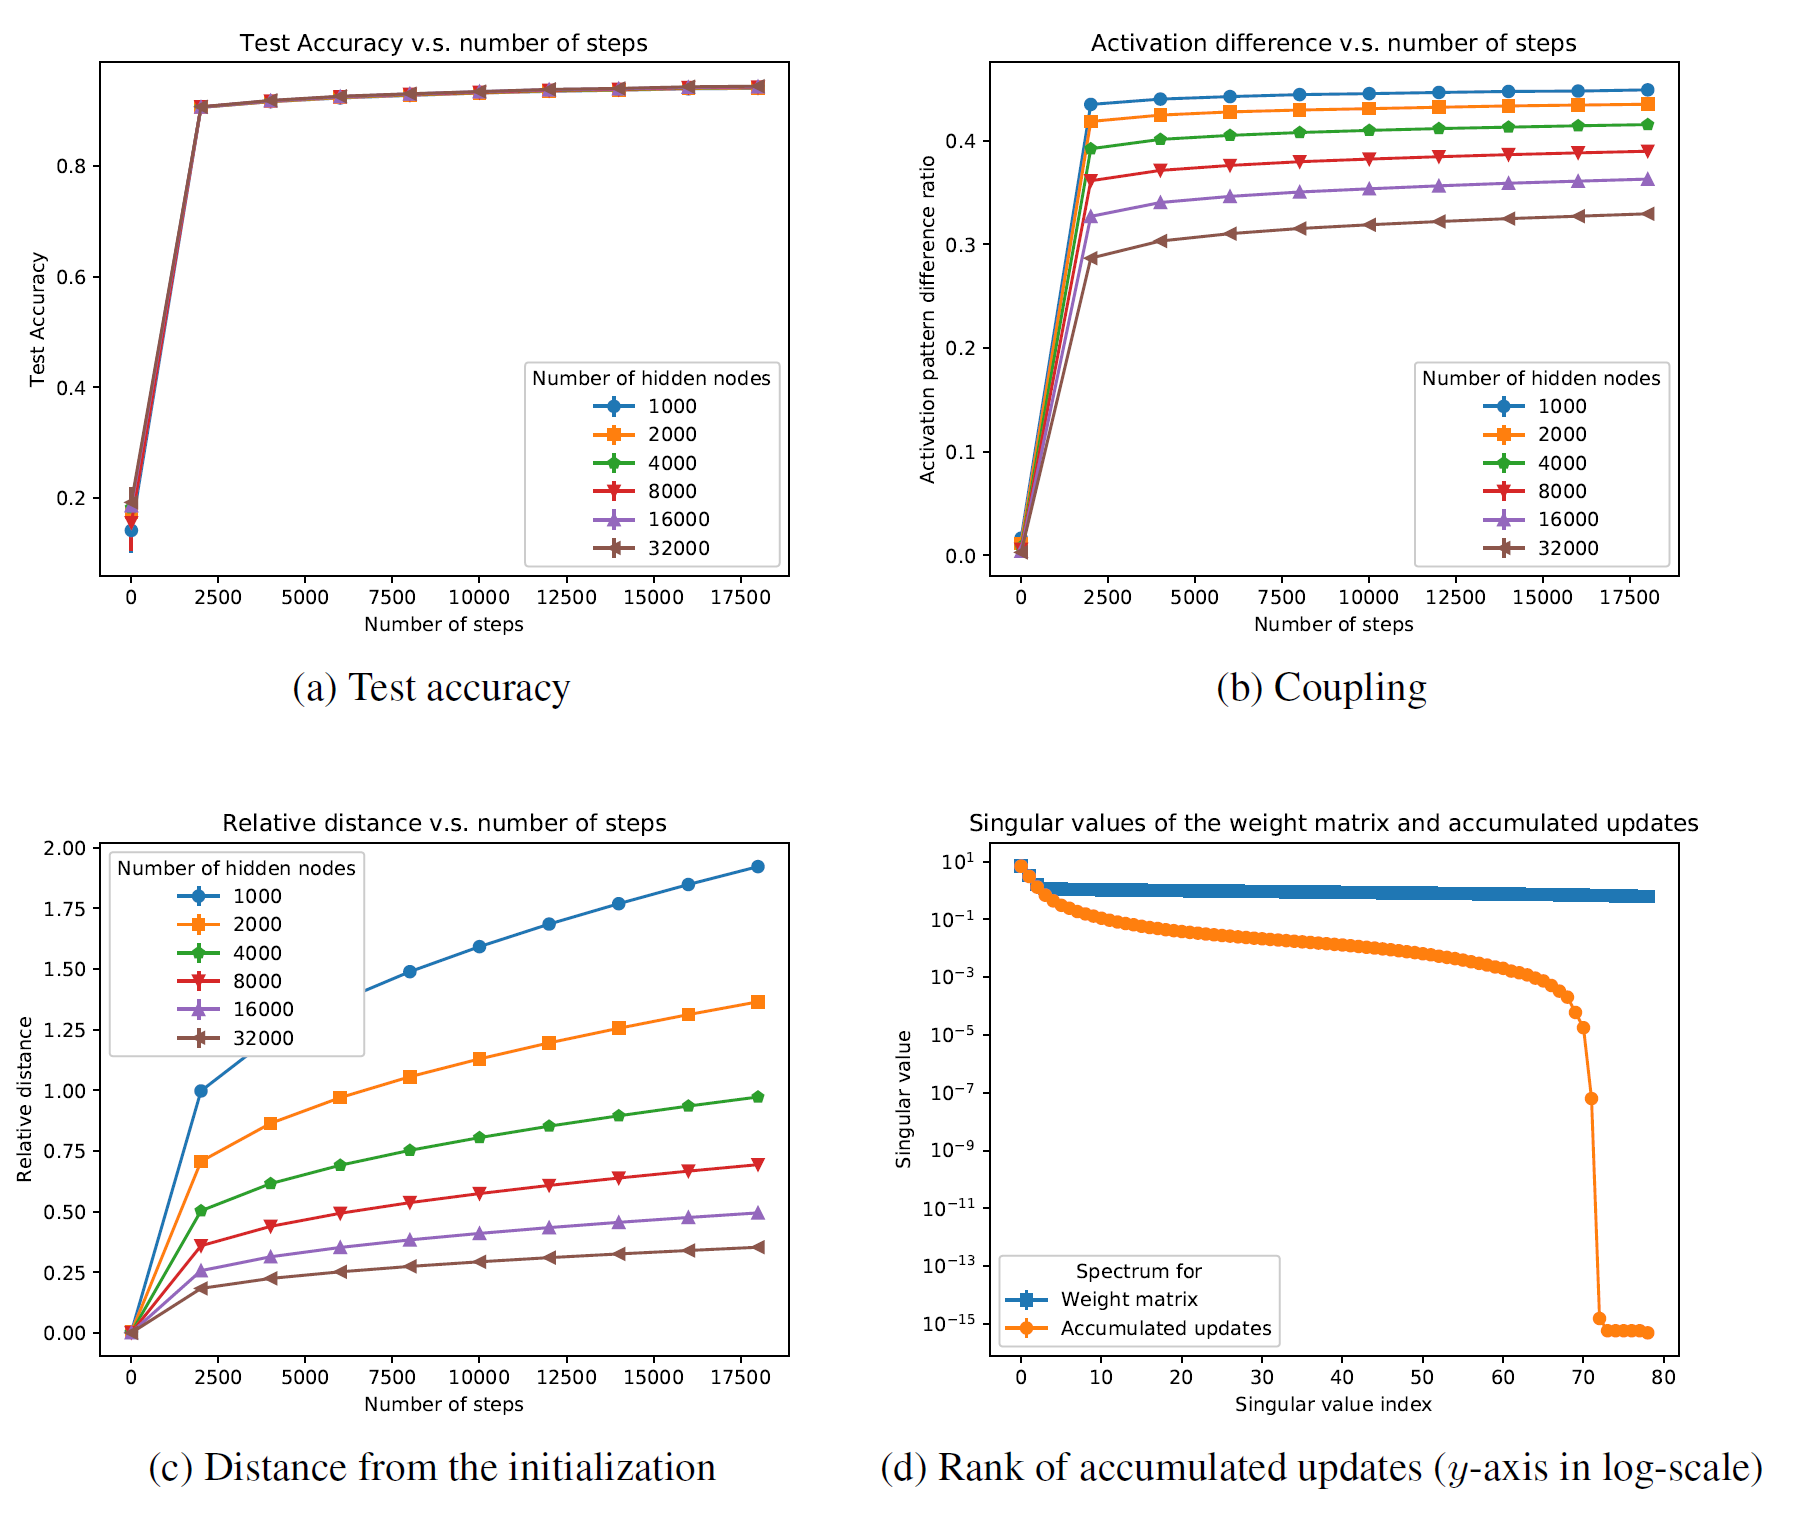
\includegraphics[width=12cm]{./figures/mnist.png}
\caption{在MNIST数据集上的结果}
\end{figure}
\par
结果。图1显示了合成数据的结果。测试精度很快收敛到100\%,隐单元数越大,测试精度越高,说明过参数化有助于优化和推广。回想一下,我们的分析表明,对于学习率随隐藏节点数$m$线性下降的情况,获得所需精度的迭代次数应该大致相同,这在这里也得到了验证。激活模式差比小于0.1,说明存在强耦合。相对距离小于0.1,因此最终的解决方案确实接近初始化。最后,累积更新的前20个奇异值比其余的大得多,而权重矩阵的谱没有这样的结构,这也与我们的分析一致。
\par
图2显示了MNIST上的结果。总体上,观察结果与合成数据上的观察结果相似(尽管不太显著),而且随着过度参数化,观察到的趋势也变得更加明显。附录中提供了一些额外的结果(例如,改变合成数据的方差),这些结果也支持我们的理论。

\section{结论}
本文研究了在实际数据集启发下,通过随机梯度下降(SGD)从随机初始化数据中学习两层超参数ReLU神经网络的问题。虽然我们的工作朝着神经网络训练的SGD的理论理解迈出了一步,但还远没有定论。特别是,对于不同于“2”的度量,甚至是某个流形给出的非凸距离,实际数据可以是可分离的。我们认为这是一个重要的开放方向。

\section{致谢}
我们要感谢NIPS'18的匿名评论员和Jason Lee的有益评论。这项工作部分得到了FA9550-18-1-0166、NSF拨款CCF-1527371、DMS-1317308、西蒙斯研究员奖、西蒙斯合作奖和ONR-N00014-16-1-2329的支持。梁颖宇也要感谢威斯康星大学麦迪逊分校研究和研究生教育副校长办公室在威斯康星校友研究基金会的资助下对这项研究的支持。
\chapter{本文重要定理及引理的证明}
\label{cha:proof}

\section{定理~\ref{theo:2:1}~的证明}\label{pr:2:1}
\begin{proof}
我们利用数学归纳法证明。
\par
对$k^\prime = 0$,显然$\|y-u(0)\|_2^2 \leq 1\cdot \|y-u(0)\|_2^2$.
\par
假设对于$k^\prime = 0,\cdots,k$,我们有$\|y-u(k^\prime)\|_2^2 \leq (1-n\lambda_0/2)^{k^\prime} \|y-u(0)\|_2^2$.
\par
对$k^\prime = k+1$,我们令
\[
A_{ir} = \{\exists w:\|w-w_r(0)\|\leq R, \mathbb{I}\{x_i^\top w_r(0)\geq 0\}\neq \mbi \{x_i^\top w\geq 0\}\}
\]
其中$R = \frac{c\lambda_0}{n^2}, c$是一个正常数。我们令$S_i = \{r\in [m]: \mbi\{A_{ir}=0\}\}, S_i^\bot  = [m]\backslash S_i\}$,则以下的引理给出了$S_i^\top$的和的大小的一个界。
\begin{lemma}
至少以概率$1-\delta$有,
\[
\sum_{i=1}^n |S_i^\top|\leq\frac{CmnR}{\delta}, C>0\makebox[3em]{为常数}
\]
\end{lemma}
\par
考虑
\[
\begin{aligned}
u_i(k+1) - u_i(k) & = \frac{1}{\sqrt{m}}\sum_{r=1}^ma_r(\sigma(w_r(k+1)^\top x_i) - \sigma (w_r(k)^\top x_i))\\
 & = \frac{1}{\sqrt{m}}\sum_{r=1}^ma_r(\sigma((w_r(k)-\eta\frac{\partial L(W(k))}{\partial w_r(k)})^\top x_i) - \sigma (w_r(k)^\top x_i))\\
\end{aligned}
\]
\par
我们利用$S_i$将上述等式的右边划分为两部分,
\[
I_1^i \triangleq \frac{1}{\sqrt{m}}\sum_{r\in S_i} a_r(\sigma((w_r(k)-\eta\frac{\partial L(W(k))}{\partial w_r(k)})^\top x_i) - \sigma (w_r(k)^\top x_i))
\]
\[
I_2^i \triangleq \frac{1}{\sqrt{m}}\sum_{r\in S_i^\bot} a_r(\sigma((w_r(k)-\eta\frac{\partial L(W(k))}{\partial w_r(k)})^\top x_i) - \sigma (w_r(k)^\top x_i))
\]
\par
因为ReLU为1-Lipschitz的,并且$|a_r| = 1$,我们有
\[
|I_2^i|\leq \frac{\eta}{\sqrt{m}} \sum_{r\in S_i^\bot }|\bigg(\frac{\partial L(W(k))}{\partial w_r(k)}\bigg)^\top x_i|\leq \frac{\eta|S_i^\bot|}{\sqrt{m}}\max_{r\in [m]}\|\frac{\partial L(W(k))}{\partial w_r(k)}\|_2\leq \frac{\eta|S_i^\bot|\sqrt{n}\|u(k)-y\|_2}{m} 
\]
\par
由于对于$\forall r\in[m]$,$\|w_r(k)-w_r(0)\|\leq R^\prime$,且$R^\prime \le R$,我们有$\mbi\{w_r(k+1)^\top x_i\geq 0\} = \mbi\{w_r(k)^\top x_i \geq 0\}, \forall r \in S_i$,则
\[
\begin{aligned}
I_1^i &= -\frac{\eta}{m}\sum_{j=1}^n x_i^\top x_j (u_j-y_j)\sum_{r\in S_i}\mbi\{w_r(k)^\top x_i\geq 0,w_r(k)^\top x_j \geq 0\}\\
 & -\eta\sum_{j=1}^n (u_j-y_j)(H_{ij}(k) - H_{ij}^\bot(k))
\end{aligned}
\]
其中$H_{ij}(k) = 1/m\sum_{r=1}^m x_i^\top x_j\mbi\{w_r(k)^\top x_i\geq 0, w_r(k)^\top x_j\geq 0\}, H_{ij}^\bot(k) = 1/m\sum_{r\in S_i^\bot} x_i^\top x_j\mbi\{w_r(k)^\top x_i\geq 0, w_r(k)^\top x_j\geq 0\}$。由上面的引理可以知道
\[
\|H*\bot(k)\|_2 \leq \sum_{(i,j)=(1,1)}^{(n,n)}|H_{ij}^\bot (k)\leq \frac{n\sum_{i=1}^n |S_i^\bot|}{m} \leq \frac{Cn^2 mR}{\delta m} \leq \frac{Cn^2R}{\delta}
\]
从而我们有
\[
\|u(k+1)-u(k)\|_2^2 \leq \eta^2\sum_{i=1}^n \frac{1}{m}\bigg(\sum_{r = 1}^m\|\frac{\partial L(W(k))}{\partial w_r(k)}\|_2 \bigg)^2\leq \eta^2 n^2\|y-u(k)\|_2^2
\]
进而通过引入交叉项有
\[
\begin{aligned}
\|y-u(k+1)\|_2^2 & = \|y-u(k) -(u(k+1)-u(k))\|_2^2\\
 & = \|y-u(k)\|_2^2 -2 (y-u(k))^\top (u(k+1)-u(k))+\|u(k+1)-u(k)\|_2^2\\
 & = \|y-u(k)\|_2^2 -2 \eta(y-u(k))^\top H(k)(y-u(k))+2\eta(y-u(k))^\top H(k)^\top (y-u(k)) \\
 & - 2(y-u(k))^\top I_2 + \|u(k+1)- u(k)\|_2^2\\
 & \leq (1-\eta\lambda_0+ \frac{2C\eta n^2R}{\delta} + \frac{2C\eta n^{3/2}R}{\delta}+eta^2 n^2)\|y-u(k)\|_2^2\\
 & \leq (1-\eta\lambda_0/2)\|y-u(k)\|_2^2
\end{aligned}
\]
其中第三个等式成立是对$u(k+1)-u(k)$的分解。
\par
由以上的结果知,对$k^\prime = k+1$命题也成立,所以由归纳法知,定理成立。
\end{proof}


\section{定理~\ref{theo:1}~的证明}\label{pr:1}
\begin{proof}
令$z_i = x_i, \theta = \sum_{l=0}^{r-1}\mathrm{S}_l^s(w)$,其中
\[
	\mathrm{S}_l^s(w) = [\underbrace{0,\cdots,0}_{ls\makebox[1em]{个}0}, w_1,\cdots,w_m,0\cdots,0]\in \mathbb{R}^d
\]
则$F_1(x_i;w) = \langle z_i,\theta \rangle$,
\par
定义$\theta\in \mathbb{R}^d$的经验范数为
\[
\|\theta\|_x^2 = \frac{1}{n}\sum_{i=1}^n |\langle z_i, \theta\rangle|^2
\]
则由于$\hat{\theta} = \sum_{l=0}^{r-1}\mathrm{S}_l^s(\hat{w})$,有
\[
	\frac{1}{n}\sum_{i=1}^n (y_i - \langle z_i, \hat{\theta}\rangle)^2 \leq \frac{1}{n}\sum_{i=1}^n (y_i - \langle z_i, {\theta}\rangle)^2
\]
又$y_i = \langle z_i, {\theta}\rangle + \varepsilon_i$,上式可以整理成为
\begin{equation}\label{eq:18}
\|\hat{\theta}- \theta\|_x^2 \leq \frac{2}{n}\sum_{i=1}^n \varepsilon_i\langle z_i,\hat{\theta}-\theta\rangle
\end{equation}
\par
设$\theta$参数的集合为$\Theta$,定义
\[
	\overline{\Theta_x} := \{\phi = \theta - \theta^\prime: \theta, \theta^\prime \in \Theta, \|\phi\|_x\leq 1\}
\]
\[
	\mathbb{G}_x(\phi) = \frac{1}{n}\sum_{i=1}^n \varepsilon_i\langle z_i,\phi\rangle
\]
则有以下引理成立
\begin{lemma}
对于参数集$\Theta$,我们有
\begin{equation}\label{eq:l4}
\sup_{\hat{\theta}\in \Theta} \sum_{i=1}^n \varepsilon_i\langle z_i,\hat{\theta}-\theta\rangle \leq \|\hat{\theta} - \theta \|_x \sup_{\phi \in \Theta_x} \sum_{i=1}^n \varepsilon_i\langle z_i,\phi\rangle
\end{equation}

\end{lemma}
\begin{proof}
为证结论成立,只需证对$\hat{\theta} \in \Theta$,有$v = (\hat{\theta} - \theta)\|\hat{\theta}-\theta\|_x \in \Theta_x$
\par
显然,$\|v\|_x \leq 1$,并且由$\theta$的定义知,$\hat{\theta}\|\hat{\theta}-\theta\|_x, \theta\|\hat{\theta}-\theta\|_x \in \Theta$,故$v\in \Theta_x$
\end{proof}
\par
将式~\ref{eq:l4}~带入式~\ref{eq:18}~中得到
\begin{equation}\label{eq:20}
\|\hat{\theta} - \theta\|_x \leq 2\cdot \sup_{\phi\in \Theta_x}\mathbb{G}_x(\phi)
\end{equation}
\par
注意到,对$\forall \phi, \phi^\prime \in \Theta_x, \mathbb{G}_x(\phi) - \mathbb{G}_x(\phi^\prime)$是次高斯随机变量,根据Dudley熵积分,有
\begin{equation}\label{eq:21}
\mathbb{E}\sup_{\phi \in \Theta_x} \mathbb{G}_x(\phi) \lesssim \frac{\sigma}{n}\int_0^\infty \sqrt{\log N(\epsilon;\Theta_x,\|\cdot\|_x)} \mathrm{d}\epsilon
\end{equation}
\par
其中,$N(\epsilon;\Theta_x,\|\cdot\|_x)$是$\Theta_x$在$\|\cdot\|_x$中的覆盖数,即满足$\sup_{\phi\in\Theta_x}\inf_{\phi^\prime \in \mathcal{H}}\|\phi-\phi^\prime\|_x \leq \epsilon$的最小集合$\mathcal{H}$的大小。
\par
将式~\ref{eq:20}~带入式~\ref{eq:21}~中得到
\begin{equation}\label{eq:22}
\mathbb{E} [\|\theta-\hat{\theta}\|_x] \lesssim \frac{\sigma}{n}\int_0^\infty \sqrt{\log N(\epsilon;\Theta_x,\|\cdot\|_x)} \mathrm{d}\epsilon
\end{equation}

\par
由于关于$\|\phi\|_x\leq 1$的性质难以推导,这里希望将其转化为$\|\phi\|_2 \leq 1$的性质的推导,由此我们引入限制特征值(restricted eigenvalues)的概念,
\begin{definition}
对于$\{z_i\}_{i=1}^n$,它对参数类$\Phi \subset \mathbb{R}^d$最小和最大限制特征值定义为
\begin{equation}\label{eq:23}
\lambda_{\min}(\{z_i\}_{i=1}^n; \Phi) := \inf_{\phi\in \Phi}\|\phi\|_x^2/\|\phi\|_2^2
\end{equation}
\begin{equation}\label{eq:24}
\lambda_{\max}(\{z_i\}_{i=1}^n; \Phi) := \inf_{\phi\in \Phi}\|\phi\|_x^2/\|\phi\|_2^2
\end{equation}
\end{definition}

\par
对$\rho > 0$,令
\[
\Theta_2(\rho) = \{\phi = \theta-\theta^\prime: \theta, \theta^\prime \in \Theta, \|\phi\|_2\leq \rho\}
\]
\par
可以证明,对于参数类$\Theta(\rho)$,可以给出限制特征值的界
\begin{lemma}
假设$\{z_i\}_{i=1}^n$为次高斯随机向量,对$\forall \rho > 0, \delta \in (*0,1/2], \epsilon\in (0,1/2]$,以下不等式以概率$1-\delta$成立
\begin{equation}
\lambda_{\min}(\{z_i\}_{i=1}^n; \Theta_2(\rho)) \geq \frac{C}{4}-O(Z\sqrt{\log(n/\delta)})\cdot \big(\epsilon + \sqrt{\frac{\log N(epsilon;\Theta_2(1),\|\cdot\|_2\log(1/\delta))}{n}}\big)
\end{equation}
\begin{equation}
\lambda_{\max}(\{z_i\}_{i=1}^n; \Theta_2(\rho)) \leq 4C-O(Z\sqrt{\log(n/\delta)})\cdot \big(\epsilon + \sqrt{\frac{\log N(epsilon;\Theta_2(1),\|\cdot\|_2\log(1/\delta))}{n}}\big)
\end{equation}
\end{lemma}
\par
因为以上得到的对限制特征值和$\|\hat{\theta}-\theta\|_x$的估计都与覆盖数有关,因此若能对覆盖数给出估计,就能得到最终的结果。


\begin{lemma}\label{le:9}
对$\forall \rho > 0, \epsilon \in (0,1]$,有以下成立
\begin{equation}
\log N(\epsilon; \Theta_2(\rho),\|\cdot\|_2) \lesssim m\log(\rho d/s)
\end{equation}
\end{lemma}

\par
通过取$\epsilon = \kappa c/C\sqrt{\log(n/\delta)}$,则可得对充分小的$\kappa > 0$,有$\epsilon \cdot O(C^2 \sqrt{\log(n/\delta)}) \leq c/16$.
\par
当
\[
	n \gtrsim c^{-1}C^2 m\cdot \log(c^{-1}Cd\log(n/\delta))\log^2(n/\delta)
\]
则以概率$1-\delta$,有
\[
	\lambda_{\min}(\{z_i\}_{i=1}^n; \Theta_2(\rho)) \geq c/8, \lambda_{\max}(\{z_i\}_{i=1}^n; \Theta_2(\rho)) \leq 8C
\]
\par
则有$c/16\|\phi\|_2^2 \leq \|\phi\|_x^2 \leq 16C\|\phi\|_2^2, \forall \phi \in \Phi$,进而有
\[
	N(\epsilon;\Theta_x,\|\cdot\|_x) \leq \log N(\epsilon/4\sqrt{C};\Theta_2(4/\sqrt{c},\|\cdot\|_2))
\]
\par
根据引理~\ref{le:9}~有
\[
\log N(\epsilon;\Theta_x,\|\cdot\|_x) \lesssim m \log(c^{-1}Cd/\epsilon)
\]
\par
将其带入式~\ref{eq:22}~并注意到
\[
	\int_0^\infty \sqrt{\max\{\log(1/\epsilon), 0\}}\mathrm{d}\epsilon = O(1)
\]
\par
则可知定理~\ref{theo:1}~成立。
\end{proof}



\section{定理~\ref{theo:2}~的证明}\label{pr:2}

\begin{proof}
为了证明下界,这里先引入以下引理
\begin{lemma}[\citet{tsybakov2008introduction}]
设$\Theta_M = (\theta_0, \theta_1, \cdots, \theta_M)$是一个有限参数集,设$P_j$为$\theta_j, j\in \{0,1,\cdots, M\}$对应的概率分布测度。设$\mathfrak{d}:\Theta_M\times \Theta_M\rightarrow \mathbb{R}^+$定义了$\Theta_M$与$\Theta_M$乘积空间上的一个半距离,并且具有以下的性质:
\begin{enumerate}
\item $\mathfrak{d}(\theta_j,\theta_k)\geq 2\rho > 0, \forall j,k\in\{0,1,\cdots,M\}$;
\item $P_j \ll P_0, \forall j \in \{1,\cdots, M\}$;
\item $\frac{1}{M}\sum_{j=1}^M KL(P_j\|P_0)\leq \gamma\log M$。 
\end{enumerate}
\par
并且以下成立,
\begin{equation}
\inf_{\hat{\theta}} \sup_{\theta_j\ in \Theta_M} \mathrm{Pr}_j[\mathfrak{d}(\hat{\theta},\theta_j)\geq \rho] \geq \frac{\sqrt{M}}{1+\sqrt{M}}(1-2\gamma-2\sqrt{\frac{\gamma}{\log M}})
\end{equation}
\end{lemma}
\par
其中$KL(\cdot,\cdot)$是两个概率分布之间的Kullback-Leibler信息量。
\par
由于在定理~\ref{theo:2}~中假设$x_i$独立同分布于正态分布,噪声也服从正态分布,因此有以下的推论:
\begin{corollary}\label{coro:13}
设$\Theta$为神经网络中的参数集合,记$\rho_{\min} = \min_{j>0}\|\theta_0- \theta_j\|_2/2$,和$\rho_{avg}^2 = \frac{1}{M}\sum_{j=1}^M \|\theta_j-\theta_0\|^2_2$,则对于任意的$n$,有
\[
\inf_{\hat{\theta}} \sup_{\theta_j\in \Theta_M} \mathbb{E}_\mu [\|\hat{\theta}_n-\theta\|_2] \geq \rho_{\min} \times\frac{\sqrt{M}}{1+\sqrt{M}}\bigg(1-\frac{n\rho_{avg}^2}{\sigma^2\log M}-2\sqrt{\frac{n\rho_{avg}^2}{2\sigma^2\log^2 M}}\bigg)
\]
\end{corollary}

\begin{lemma}\label{le:14}
设$\Theta \in \mathbb{R}^d$为神经网络参数集,$\mathcal{I}\subset [d]=\{1,2,\cdots,d\}$,设对任意的$u \in \mathbb{R}^{|\mathcal{I}|}$存在$\theta\in \Theta$使得$u$为$\theta$在$\mathcal{I}$维度上的限制,则存在推论中的有限子集$\Theta^\prime \subset \Theta$,使得$\log M \asymp |\mathcal{I}|, \rho_{\min} \asymp \rho_{avg} \asymp \sqrt{|\mathcal{I}|}\epsilon, \forall \epsilon > 0$.
\end{lemma}
\par
下面的引理说明$\theta$的前$m$个组成成分为自由变量。
\begin{lemma}\label{le:15}
设$\mathcal{I} = \{1,\cdots,m\}$,则对任意的$u\in \mathbb{R}^m$,存在$\theta \in \Theta$满足$\theta|_{\mathcal{I}} = u$
\end{lemma}

\par
令$\epsilon \asymp \sigma \sqrt{m/n}$,则由引理~\ref{le:14}~和~\ref{le:15}~以及推论~\ref{coro:13}~知,定理~\ref{theo:2}~成立。

\end{proof}



\end{appendix}

%% 个人简历
\begin{resume}

  \resumeitem{个人简历}

  xxxx 年 xx 月 xx 日出生于 xx 省 xx 县。

  xxxx 年 9 月考入 xx 大学 xx 系 xx 专业,xxxx 年 7 月本科毕业并获得 xx 学士学位。

  xxxx 年 9 月免试进入 xx 大学 xx 系攻读 xx 学位至今。

  \researchitem{发表的学术论文} % 发表的和录用的合在一起

  % 1. 已经刊载的学术论文(本人是第一作者,或者导师为第一作者本人是第二作者)
  \begin{publications}
    \item Yang Y, Ren T L, Zhang L T, et al. Miniature microphone with silicon-
      based ferroelectric thin films. Integrated Ferroelectrics, 2003,
      52:229-235. (SCI 收录, 检索号:758FZ.)
    \item 杨轶, 张宁欣, 任天令, 等. 硅基铁电微声学器件中薄膜残余应力的研究. 中国机
      械工程, 2005, 16(14):1289-1291. (EI 收录, 检索号:0534931 2907.)
    \item 杨轶, 张宁欣, 任天令, 等. 集成铁电器件中的关键工艺研究. 仪器仪表学报,
      2003, 24(S4):192-193. (EI 源刊.)
  \end{publications}

  % 2. 尚未刊载,但已经接到正式录用函的学术论文(本人为第一作者,或者
  %    导师为第一作者本人是第二作者)。
  \begin{publications}[before=\publicationskip,after=\publicationskip]
    \item Yang Y, Ren T L, Zhu Y P, et al. PMUTs for handwriting recognition. In
      press. (已被 Integrated Ferroelectrics 录用. SCI 源刊.)
  \end{publications}

  % 3. 其他学术论文。可列出除上述两种情况以外的其他学术论文,但必须是
  %    已经刊载或者收到正式录用函的论文。
  \begin{publications}
    \item Wu X M, Yang Y, Cai J, et al. Measurements of ferroelectric MEMS
      microphones. Integrated Ferroelectrics, 2005, 69:417-429. (SCI 收录, 检索号
      :896KM)
    \item 贾泽, 杨轶, 陈兢, 等. 用于压电和电容微麦克风的体硅腐蚀相关研究. 压电与声
      光, 2006, 28(1):117-119. (EI 收录, 检索号:06129773469)
    \item 伍晓明, 杨轶, 张宁欣, 等. 基于MEMS技术的集成铁电硅微麦克风. 中国集成电路,
      2003, 53:59-61.
  \end{publications}

  \researchitem{研究成果} % 有就写,没有就删除
  \begin{achievements}
    \item 任天令, 杨轶, 朱一平, 等. 硅基铁电微声学传感器畴极化区域控制和电极连接的
      方法: 中国, CN1602118A. (中国专利公开号)
    \item Ren T L, Yang Y, Zhu Y P, et al. Piezoelectric micro acoustic sensor
      based on ferroelectric materials: USA, No.11/215, 102. (美国发明专利申请号)
  \end{achievements}

\end{resume}


%% 本科生进行格式审查是需要下面这个表格,答辩可能不需要。选择性留下。
% 综合论文训练记录表
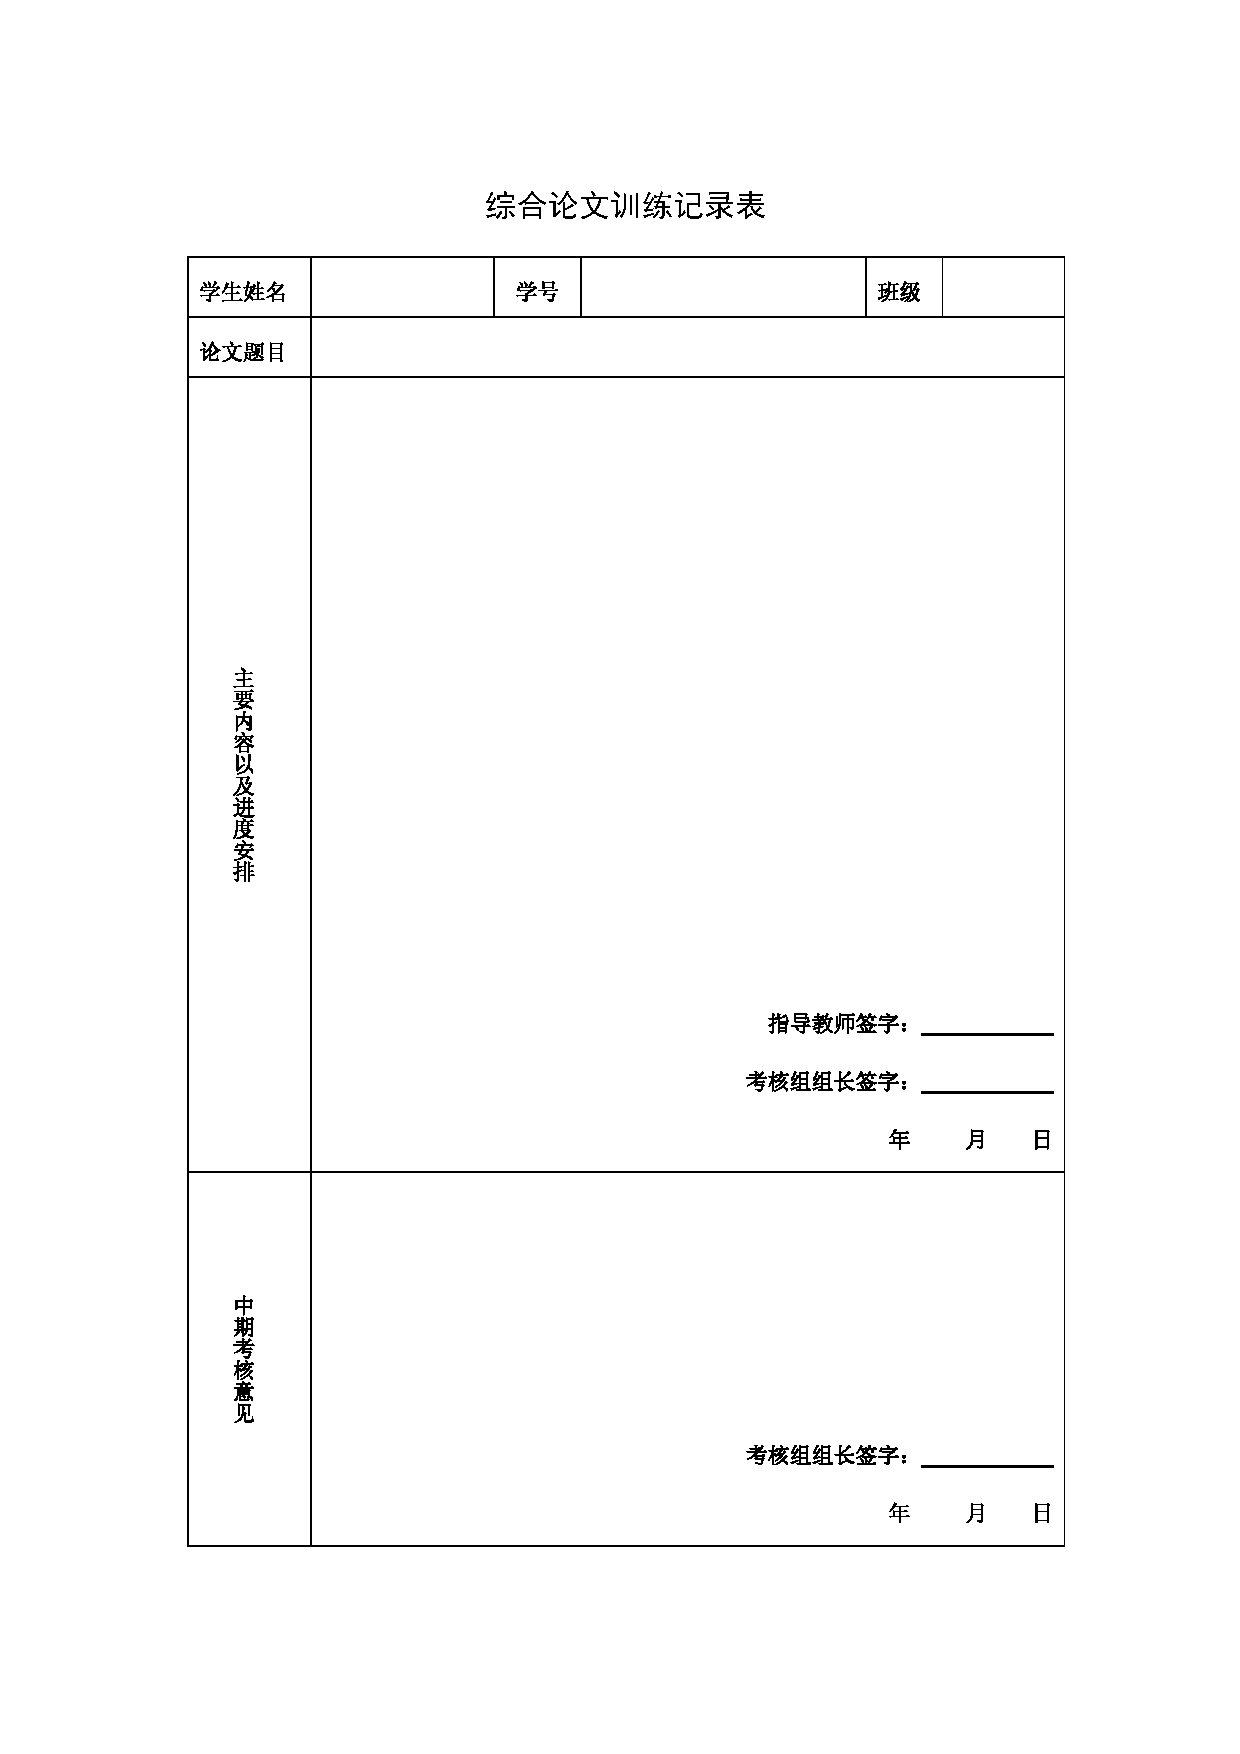
\includepdf[pages=-]{scan-record.pdf}
\end{document}
